%\documentclass[utf8,zihao=-4,aspectratio=1610]{ctexbeamer}
\documentclass[utf8,zihao=-4,handout,smaller,aspectratio=1610]{ctexbeamer}
\usepackage{multimedia}
\usepackage{hyperref}
\usepackage{smartdiagram}
\usepackage{listings}
\usepackage{tikz}
\usetikzlibrary{shapes.geometric,calc}
\usesmartdiagramlibrary{additions} 
\setbeamercovered{highly dynamic}

%% 所要粘贴代码的编程语言
%\lstloadlanguages{}

%% 设置listings宏包的一些全局样式
%% 参考http://hi.baidu.com/shawpinlee/blog/item/9ec431cbae28e41cbe09e6e4.html
\lstset{
	showstringspaces=false, %设定是否显示代码之间的空格符号
	numbers=left,% 在左边显示行号
	numberstyle=\tiny, % 设定行号字体的大小
	basicstyle=\footnotesize,% 设定字体大小\tiny, \small, \large等等
	keywordstyle=\color{blue!70}, commentstyle=\color{red!50!green!50!blue!50},% 关键字高亮
	frame=shadowbox, % 给代码加框
	rulesepcolor=\color{red!20!green!20!blue!20},
	escapechar=`, % 中文逃逸字符,用于中英混排
	xleftmargin=2em,xrightmargin=2em, aboveskip=1em,
	breaklines,% 这条命令可以让latex自动将长的代码行换行排版
	extendedchars=false % 这一条命令可以解决代码跨页时,章节标题,页眉等汉字不显示的问题
}

\usetheme{madrid}
%\useoutertheme{miniframes}

\usecolortheme{orchid}
\title{ 孔加工概述~~说课}
\author{高星}
\institute{湖南潇湘技师学院~湖南九嶷职院}
\date{2017.12.1}
\begin{document}
\section*{封面}    
\begin{frame}[plain]
	\maketitle
	\noindent
    
	\centering	\begin{tabular}[t]{*{4}{l@{~ }}}
			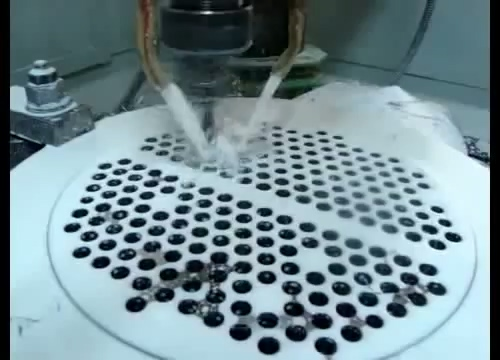
\includegraphics[width=0.22\linewidth,trim=0 0 0 0,clip,angle=0]{image/1.jpg} & 
			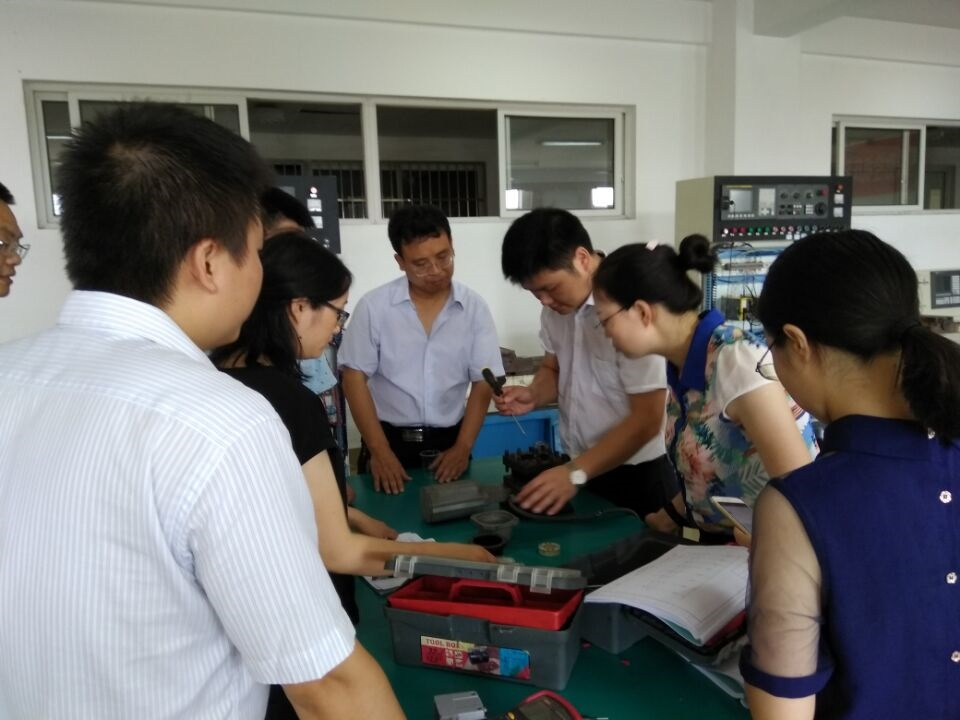
\includegraphics[width=0.22\linewidth,trim=300 1.5cm 0 7cm,clip,angle=0]{image/2.jpg}&
			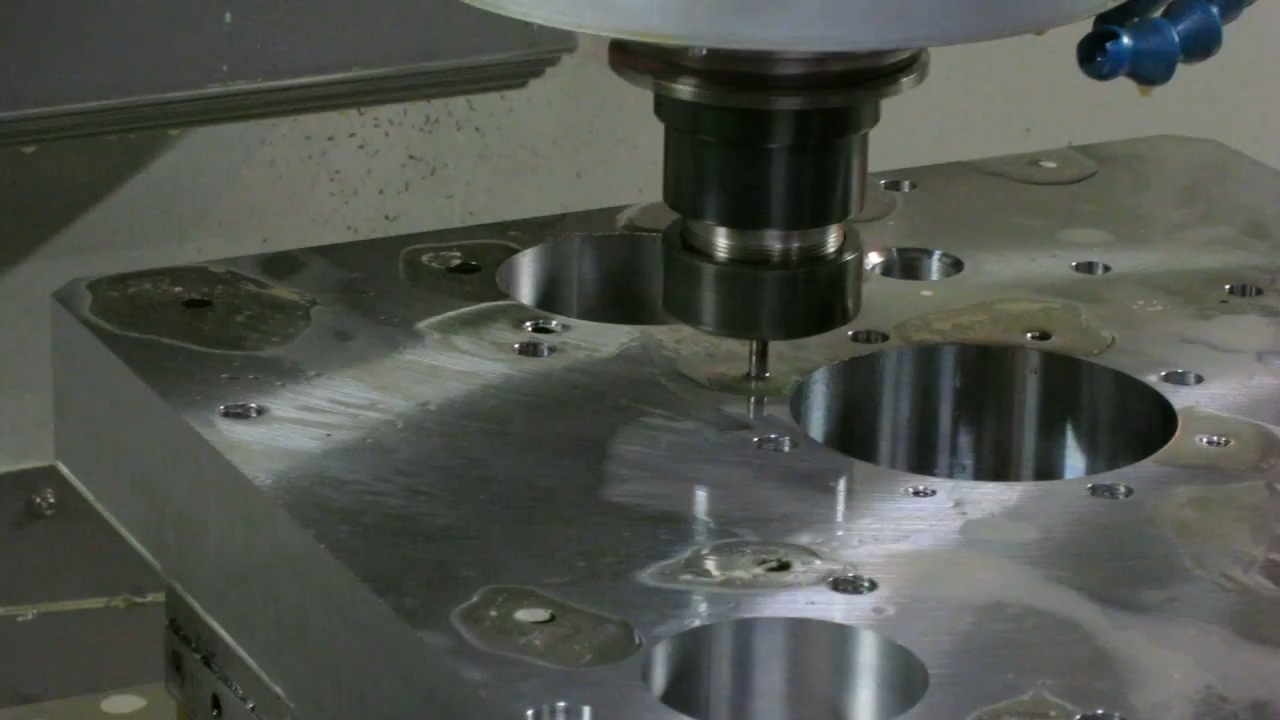
\includegraphics[width=0.22\linewidth,trim=10cm 0 0 0,clip,angle=0]{image/3.jpg}&
			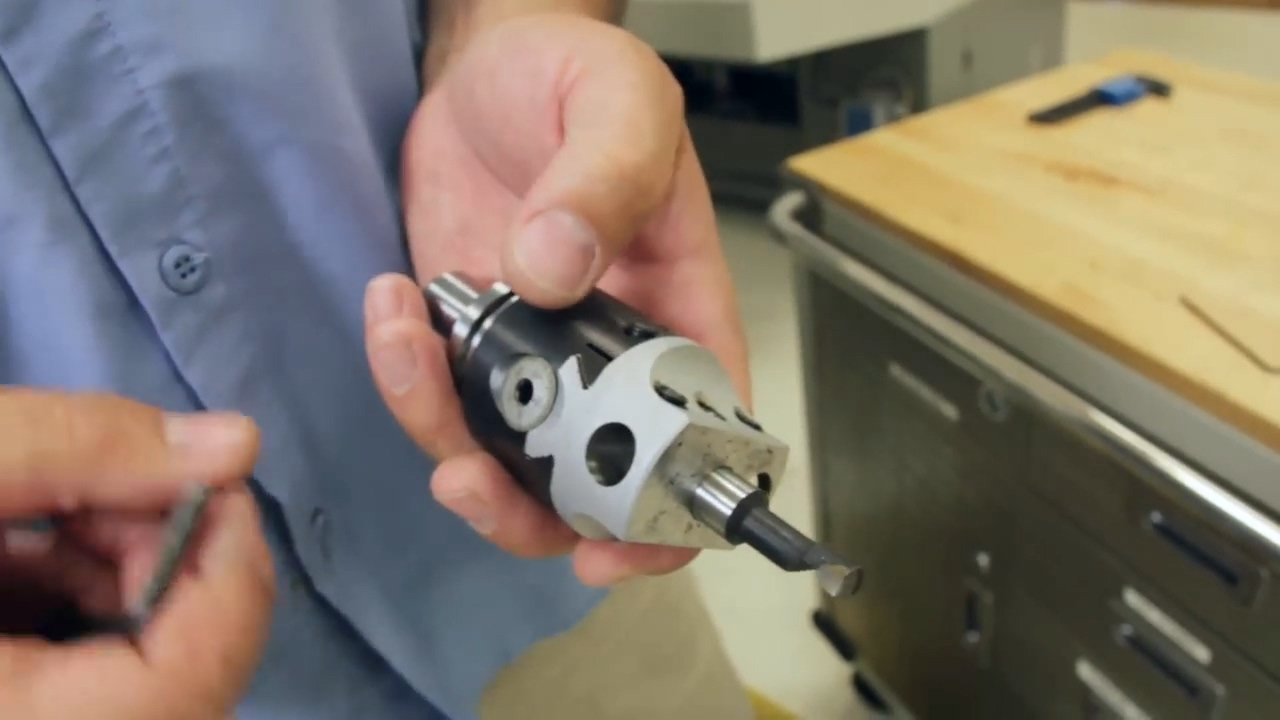
\includegraphics[width=0.22\linewidth,trim=10cm 0  0 0,clip,angle=0]{image/4.jpg}
	\end{tabular}
\vfill 

\end{frame}

\section*{目录}    
\begin{frame}{说课内容}
    \begin{columns}[onlytextwidth]
        \column[c]{0.1\textwidth}	
        \column[c]{0.3\textwidth}
        \tableofcontents[hideallsubsections]
        \column[c]{0.6\textwidth}
        \vspace{0.5cm}
        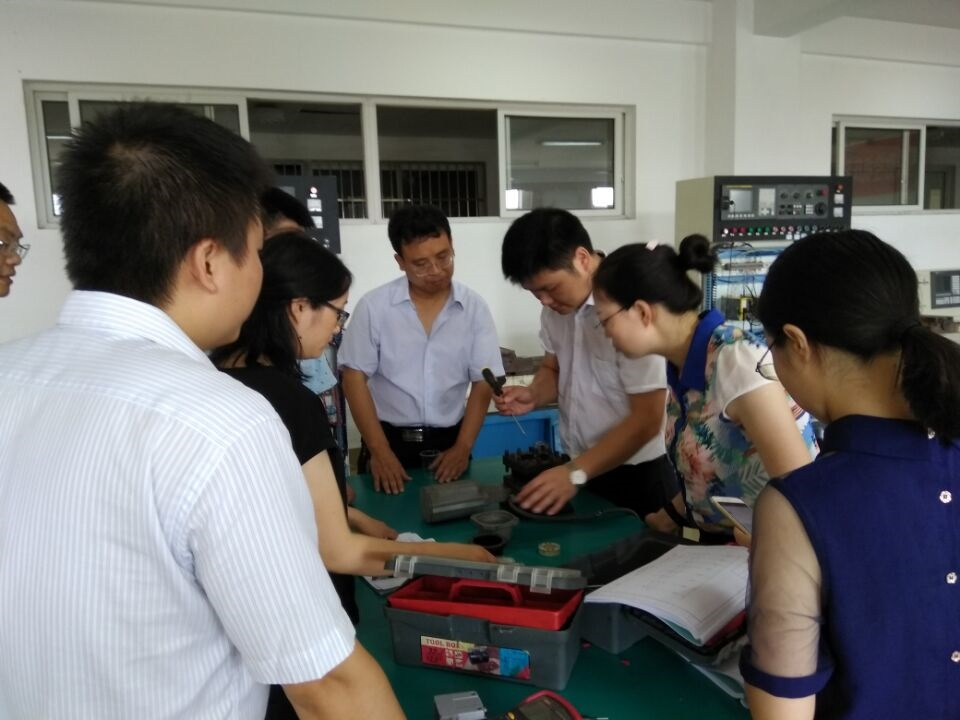
\includegraphics[width=0.9\linewidth,trim=0 0 0 0,clip,angle=0]{image/2.jpg}
    \end{columns}
\end{frame}

\section{说教材}
\subsection{教材选择}
\begin{frame}{教材选择}
	\begin{columns}[onlytextwidth]
		\column{.5\textwidth}

\begin{enumerate}
   \item<1-> 教材:《数控机床编程与操作(数控铣床/加工中心分册)》,中国劳动出版社,沈建峰     
     
\end{enumerate}
    \onslide<2-> 
\smartdiagramset{border color=black,%边界颜色
   	set color list={blue!50!cyan,green!60!lime,orange!50!red,red!80!black},%颜色列表
    module x sep=5cm,%向间距
    module y sep=1.5cm,%向间距
    uniform arrow color=true,%是否制定颜色
    arrow color=white,%箭头颜色
    arrow line width=0.5cm,%箭头宽度
   	back arrow disabled=true,%是否箭头返回
%   module minimum width=5cm,%最小宽度
%module minimum height=2cm,%最小高度
text width=4cm,%文本宽度
}
  \begin{center}
       \smartdiagram[flow diagram]{出版社重视技能,与本学校系统相同}
  \end{center}     

	\column{.5\textwidth}
    \onslide<1->
\includegraphics[width=0.9\linewidth,trim=0 0 0 0,clip,angle=0]{image/5.jpg}
	\end{columns}
\end{frame}

\begin{frame}{参考书}
	 \begin{itemize}
	 	\item<1->《国家职业标准------加工中心操作工》,劳动社会保障出版社
	 	\item<2->《加工中心编程与操作》,科学出版社,主编刘加孝 
	 	\item<3->《数控铣削宏程序及应用实例》,机械工业出版社,陈海舟
	 	\item<4-> 《Fanuc 编程说明书》、《数控加工工艺》

	 	
	 \end{itemize}
% \centering
 \hspace{2cm}\includegraphics<1->[width=0.22\linewidth,trim=0 0 0 0,clip,angle=0]{image/7.jpg}~~ 
 \includegraphics<2->[width=0.22\linewidth,trim=0 0 0  0,clip,angle=0]{image/6.jpg}~~
\includegraphics<3->[width=0.22\linewidth,trim=0 0 0 0,clip,angle=0]{image/8.jpg} 
 
\end{frame}






\subsection{教材中的位置与地位}
\begin{frame}{教材中的位置与地位}
 	\begin{columns}[onlytextwidth]
 	\column{.4\textwidth}
 	 \begin{itemize}
 		\item<1->《国家职业标准------加工中心操作》手工编程必考内容
 		
 		\item<2->比赛手工编程四大结构之一
 		
 		\item<3-> 教材第二章第三节、第四章第三节
 		\item<4-> 教材处理
	\end{itemize}
 	\column{.6\textwidth}
\begin{center}
\smartdiagramset{border color=black,%边界颜色
    set color list={blue!50!cyan,green!60!lime,orange!50!red,red!80!black,blue!50!cyan,green!60!lime,orange!50!red,red!80!black},%颜色列表
    module x sep=5cm,%向间距
    module y sep=1.5cm,%向间距
    uniform arrow color=true,%是否制定颜色
    arrow color=white,%箭头颜色
    arrow line width=0.5cm,%箭头宽度
    back arrow disabled=true,%是否箭头返回
    %   module minimum width=5cm,%最小宽度
    %module minimum height=2cm,%最小高度
    text width=8cm,%文本宽度
    bubble fill opacity=0
}
\scalebox{0.7}{
\smartdiagram[connected constellation diagram]{数控铣编\\程与操作,基本知识,平面加工,外形加工,挖槽加工,孔加工,简化编程}%中心主题
}

\end{center}

	\end{columns}    
\end{frame}

\subsection{主题安排}
\begin{frame}{主题安排}
	\begin{columns}[onlytextwidth]
	\column{\textwidth}
       \begin{center}
        \smartdiagramset{border color=black,%边界颜色
            set color list={blue!50!cyan,green!60!lime,orange!50!red,red!80!black,blue!50!cyan,green!60!lime,orange!50!red,red!80!black},%颜色列表
            module x sep=5cm,%向间距
            module y sep=1.5cm,%向间距
            uniform arrow color=true,%是否制定颜色
            arrow color=white,%箭头颜色
            arrow line width=0.5cm,%箭头宽度
            back arrow disabled=true,%是否箭头返回
            %   module minimum width=5cm,%最小宽度
            %module minimum height=2cm,%最小高度
            text width=8cm,%文本宽度
            bubble fill opacity=0
        }
        \scalebox{0.7}{
            \smartdiagram[connected constellation diagram]{孔加工,孔加工概述\\(2节),Fanuc孔加工编程及工艺\\(2节),Fanuc孔系编程\\(2节),Siemen孔加工编程\\(2节),仿真及机床操作\\(18节)}%中心主题
        }
    \end{center}
    \column{0\textwidth}
%    \begin{itemize}
%    	\item<1-> 前面学习了挖槽加工,其中有圆形槽加工。
%    	\item<2-> 后面要学Fanuc、Siemens孔加工固定循环。
%    	\item<3-> 孔加概述承前启后主要为后面的学习打基础。
%    \end{itemize}
 \end{columns}  
\end{frame}

\subsection{主题分析}
\begin{frame}{主题分析}
	\begin{columns}[onlytextwidth]
	\column{.1\textwidth}
	\column{.8\textwidth}
	\begin{itemize}
		\item<1-> 前面学习了挖槽加工,其中有圆形槽加工。
		\item<2-> 后面要学Fanuc、Siemens孔加工固定循环。
		\item<3-> 孔加工概述承前启后主要为后面的学习打基础。
	\end{itemize}
   \vspace{0.5cm}
	\includegraphics<1->[width=0.33\linewidth,trim=400 300 600 400,clip,angle=0]{image/9.jpg}~~ 
	\includegraphics<2->[width=0.33\linewidth,trim=0 0 0  0,clip,angle=0]{image/1.jpg}~~
	\includegraphics<3->[width=0.33\linewidth,trim=10cm 0 0 0,clip,angle=0]{image/3.jpg}
	\column{.1\textwidth}
	 \end{columns}
\end{frame}

\subsection{教学目标}
\begin{frame}{教学目标}
 \begin{columns}[onlytextwidth]
    \column{.15\textwidth}
    \column{.7\textwidth}
    \begin{block}{知识目标}
        \begin{enumerate}[<+->]
            \item 掌握孔加工的方式;
            \item 掌握传统孔加工的刀具;
            \item 了解铣孔与传统孔加工的区别;
            \item 掌握孔加工的6个动作与3个平面;
            \item 能结合子程序编写孔加工程序;
        \end{enumerate}
    \end{block}
    \column{.15\textwidth}
 \end{columns}
\end{frame}

\begin{frame}{教学目标}
	\begin{columns}[onlytextwidth]
		\column{.0\textwidth}
	
		\column{.4\textwidth}
	\begin{block}{能力目标}
	\begin{enumerate}
		\item 总结能力提升;
		\item 找资料自我学习提升;
		\item 找规律及编程能力提升;
		\item 表达能力提升;
	\end{enumerate}
\end{block}
		\column{.5\textwidth}
				\begin{block}{情感目标}
			\begin{enumerate}
				\item 增长见识,激发学习兴趣;
				\item 意识到做事要认真,一丝不苟;
				\item 意识到6S规范及习惯的必要性;
				\item 增加安全意识;
			\end{enumerate}
		\end{block}
		\column{.0\textwidth}
	\end{columns}
\end{frame}

\subsection{重点难点}
\begin{frame}{重点难点}
 \begin{columns}[onlytextwidth]
	\column{.1\textwidth}
	\column{.8\textwidth}
	        \smartdiagramset{border color=black,%边界颜色
		set color list={blue!50!cyan,green!60!lime,orange!50!red,red!80!black,blue!50!cyan,green!60!lime,orange!50!red,red!80!black},%颜色列表
		module x sep=5cm,%向间距
		module y sep=1.5cm,%向间距
		uniform arrow color=true,%是否制定颜色
		arrow color=white,%箭头颜色
		arrow line width=0.5cm,%箭头宽度
		back arrow disabled=true,%是否箭头返回
		%   module minimum width=5cm,%最小宽度
		%module minimum height=2cm,%最小高度
		text width=8cm,%文本宽度
		bubble fill opacity=0
	}
\centering \smartdiagram[flow diagram]{孔加工的方式,编写孔加工程序}%垂直流线。

	\column{.2\textwidth}
\end{columns}
\end{frame}

\section{说学法}
\begin{frame}{说学法}
	\begin{columns}[onlytextwidth]
		\column{0\textwidth}
		\column{\textwidth}
	\centering	\includegraphics<1->[width=0.8\linewidth,trim=0 0 0 0,clip,angle=0]{image/10.jpg}
		\column{0\textwidth}
	\end{columns}
\end{frame}


\section{说教法}
\begin{frame}{说教法}
    \begin{columns}
        \column{0.5\textwidth}
        \smartdiagram[circular diagram]{多媒体演示法,讲解分析法,实物展示法}%圆形,逆时针。              
        \column{0.5\textwidth}
\flushright  \smartdiagram[circular diagram:clockwise]{课外作业考核,仿真作业考核,实习课题考核}%圆形,逆时针。                
        \column{0\textwidth}
    \end{columns}
\end{frame}

\section{说教学过程}
\subsection*{教学整体过程}
\begin{frame}{说教学过程}
	
    \begin{columns}[onlytextwidth]
       \smartdiagramset{border color=black,%边界颜色
    	set color list={blue!50!cyan,green!60!lime,orange!50!red,red!80!black,blue!50!cyan,green!60!lime,orange!50!red,red!80!black},%颜色列表
    	module x sep=5cm,%向间距
    	module y sep=1.3cm,%向间距
    	uniform arrow color=true,%是否制定颜色
    	arrow color=white,%箭头颜色
    	arrow line width=0.5cm,%箭头宽度
    	back arrow disabled=true,%是否箭头返回
    	%   module minimum width=5cm,%最小宽度
    	module minimum height=4cm,%最小高度
    	text width=3cm,%文本宽度
    	bubble fill opacity=0
    }	
        \column{0.2\textwidth}
\centering \smartdiagram[flow diagram]{组织教学\\复习(5')。}        
\column{0.3\textwidth}
       \smartdiagramset{border color=black,%边界颜色
	set color list={blue!50!cyan,green!60!lime,orange!50!red,red!80!black,blue!50!cyan,green!60!lime,orange!50!red,red!80!black},%颜色列表
	module x sep=5cm,%向间距
	module y sep=1.3cm,%向间距
	uniform arrow color=true,%是否制定颜色
	arrow color=white,%箭头颜色
	arrow line width=0.5cm,%箭头宽度
	back arrow disabled=true,%是否箭头返回
	%   module minimum width=5cm,%最小宽度
	module minimum height=1cm,%最小高度
	text width=6cm,%文本宽度
	bubble fill opacity=0
}	
\centering \smartdiagram[flow diagram]{%垂直流线。
孔加工的方式(25'),
传统孔加工的刀具(10'),
铣孔与传统孔加工的区别(10'),
孔加工的6个动作与3个平面(10'),
能结合子程序编写孔加工程序(25')}  
  
      \column{0.33\textwidth}
      
\flushright \smartdiagram[flow diagram]{小结、作业布置(5')}  
         
    \end{columns}
\end{frame}

\subsection*{教学过程}
\begin{frame}{组织教学、复习}
	\begin{columns}
		\column{0.1\textwidth}
		\column{0.5\textwidth}
\begin{enumerate}
	\item <1->集中注意力、清点人数;
		
		\item <1->圆槽的加工思路与路径;
		
	\item <2->子程序的编程Z向分层的思路;  
\end{enumerate}
		
	\pause	
		
		\column{2\textwidth}
		\begin{itemize}
			\item<1-> 本节课后面要用到;  
		\end{itemize}
	\end{columns}

\vspace{0.5cm}

~~~~~~~~~~~~~~~~	\includegraphics<1->[width=0.29\linewidth,trim=0 0 0 0,clip,angle=0]{image/11.jpg} ~~~~
	\includegraphics<2->[width=0.33\linewidth,trim=0 0 0 0,clip,angle=0]{image/12.jpg}

\end{frame}

\begin{frame}{孔加工方式}
	\begin{columns}
		\column{0\textwidth}
		\column{.5\textwidth}
			
		\begin{itemize}
			\item 教学方法:多媒体演示法
		
		\item 有目的的观看,提问:
	
		\begin{enumerate}
			\item 有哪些孔加工方式?
		\item 有哪些刀具?
		\item 孔加工过程?
		\end{enumerate}
			\end{itemize}
		\column{.5\textwidth}
		
		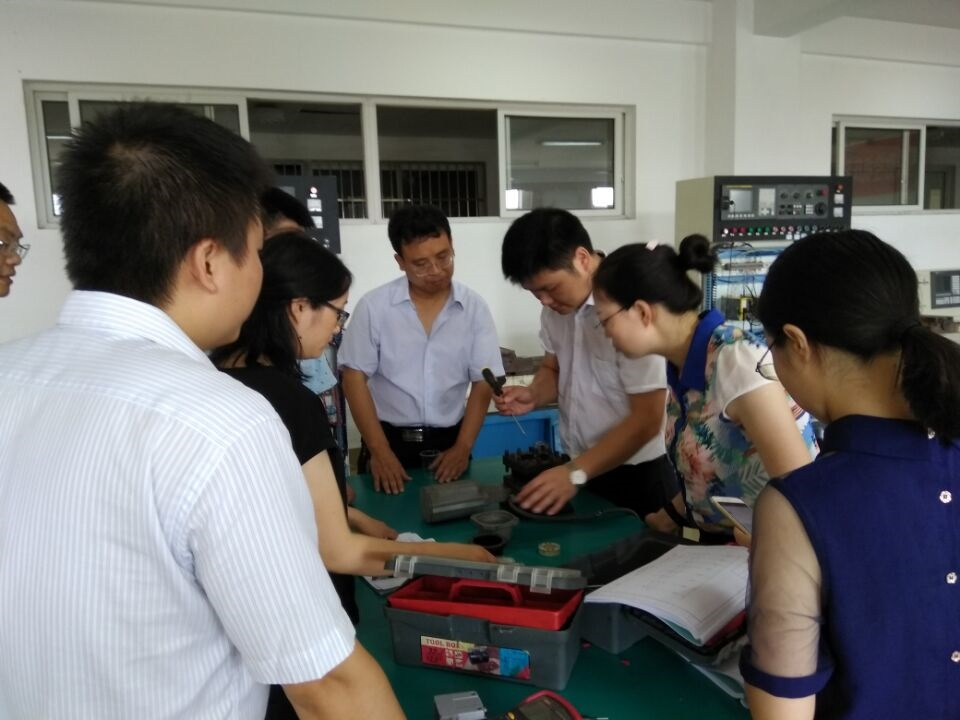
\includegraphics[width=0.9\linewidth,trim=0 0 0 0,clip,angle=0]{image/2.jpg}
		
	\end{columns}
\end{frame}

\begin{frame}{孔加工方式}
	\begin{columns}
		\column{.05\textwidth}
		\column{.7\textwidth}
\begin{block}{视频内容选择}
	\begin{itemize}
	\item 知识内容:中心孔、钻孔,镗孔、铰孔、攻丝。
	\item 扩展内容:钻方孔,分割钻。
	\item 工厂现场:6S要求讲解,别人的习惯。
	\item 安全意识:有安全隐患的视频。
	\end{itemize}
	|\end{block}		
	
		\column{.0\textwidth}
	\end{columns}
\end{frame}

\begin{frame}{孔加工方式}
	\begin{columns}
		\column{.05\textwidth}
		\column{.7\textwidth}
		\begin{block}{知识内容:}
				  中心孔、钻孔,镗孔、铰孔、攻丝。
			|\end{block}

		\column{.0\textwidth}
	\end{columns}

\vspace{25pt}

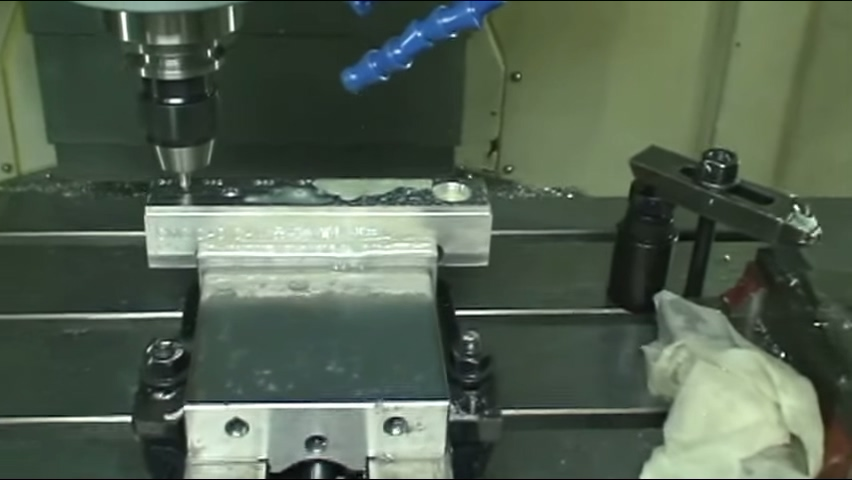
\includegraphics[width=0.5\linewidth,trim=0 0 0 0,clip,angle=0]{image/zhongxingkong.jpg}~
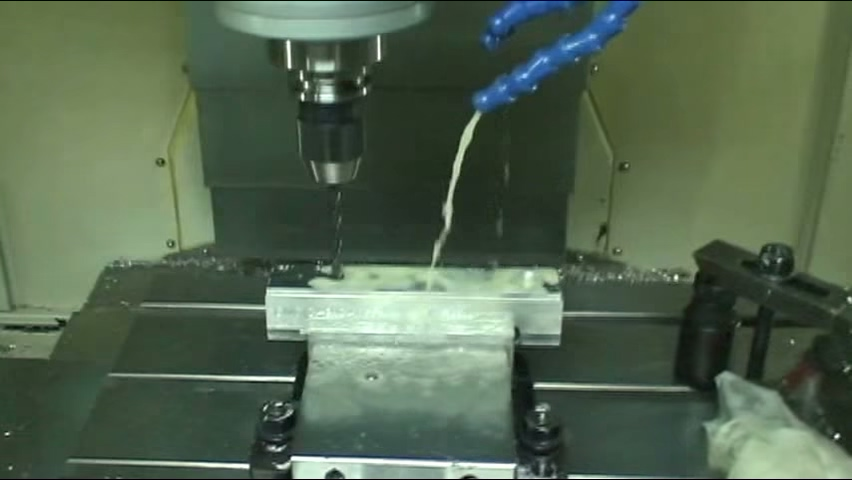
\includegraphics[width=0.5\linewidth,trim=0 0 0 0,clip,angle=0]{image/zuankong.jpg}

\end{frame}

\begin{frame}{孔加工方式}
	\begin{columns}
		\column{.05\textwidth}
		\column{.6\textwidth}
		\begin{block}{知识内容:}
			中心孔、钻孔,镗孔、铰孔、攻丝。
			|\end{block}
		\column{.0\textwidth}
	\end{columns}

\vspace{25pt}

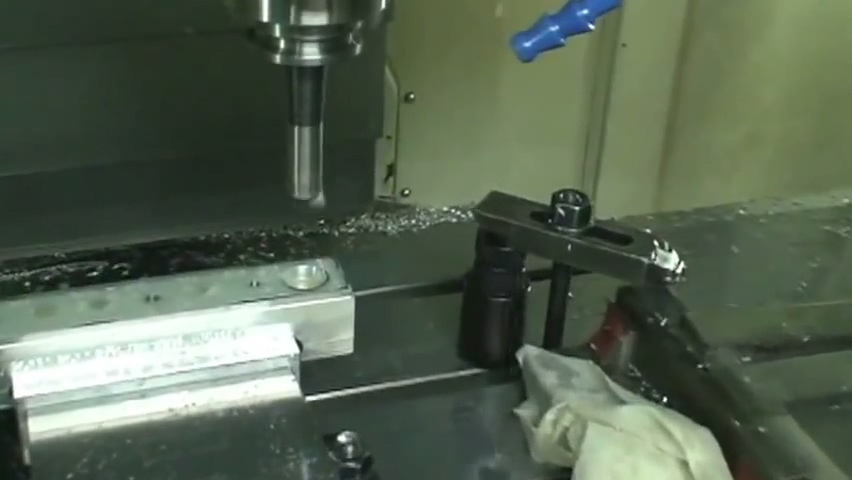
\includegraphics[width=0.5\linewidth,trim=0 0 0 0,clip,angle=0]{image/tang.jpg}~
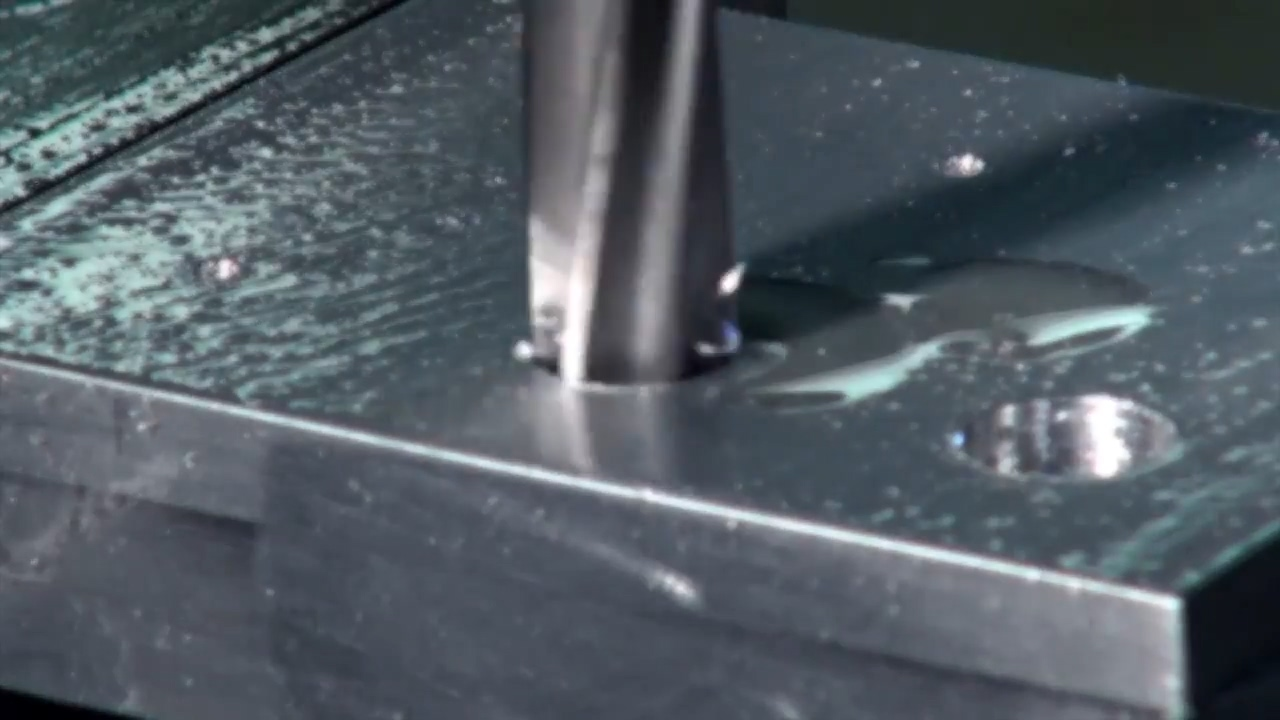
\includegraphics[width=0.5\linewidth,trim=0 0 0 0,clip,angle=0]{image/jiaokong.jpg}
	
\end{frame}

\begin{frame}{孔加工方式}
	\begin{columns}
		\column{.05\textwidth}
		\column{.6\textwidth}
		\begin{block}{知识内容:}
			中心孔、钻孔,镗孔、铰孔、攻丝。
			|\end{block}
		\column{.0\textwidth}
	\end{columns}
	
	\vspace{25pt}
	
	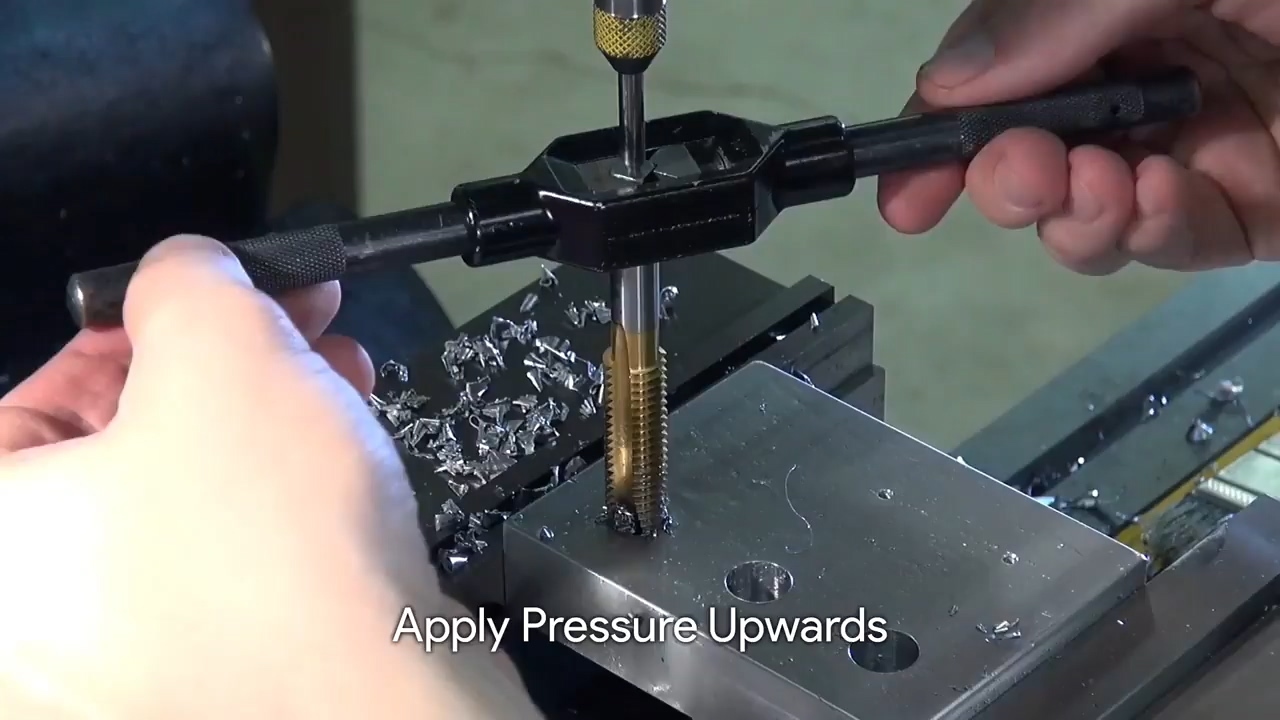
\includegraphics[width=0.5\linewidth,trim=0 0 0 0,clip,angle=0]{image/shougongsi.jpg}~
	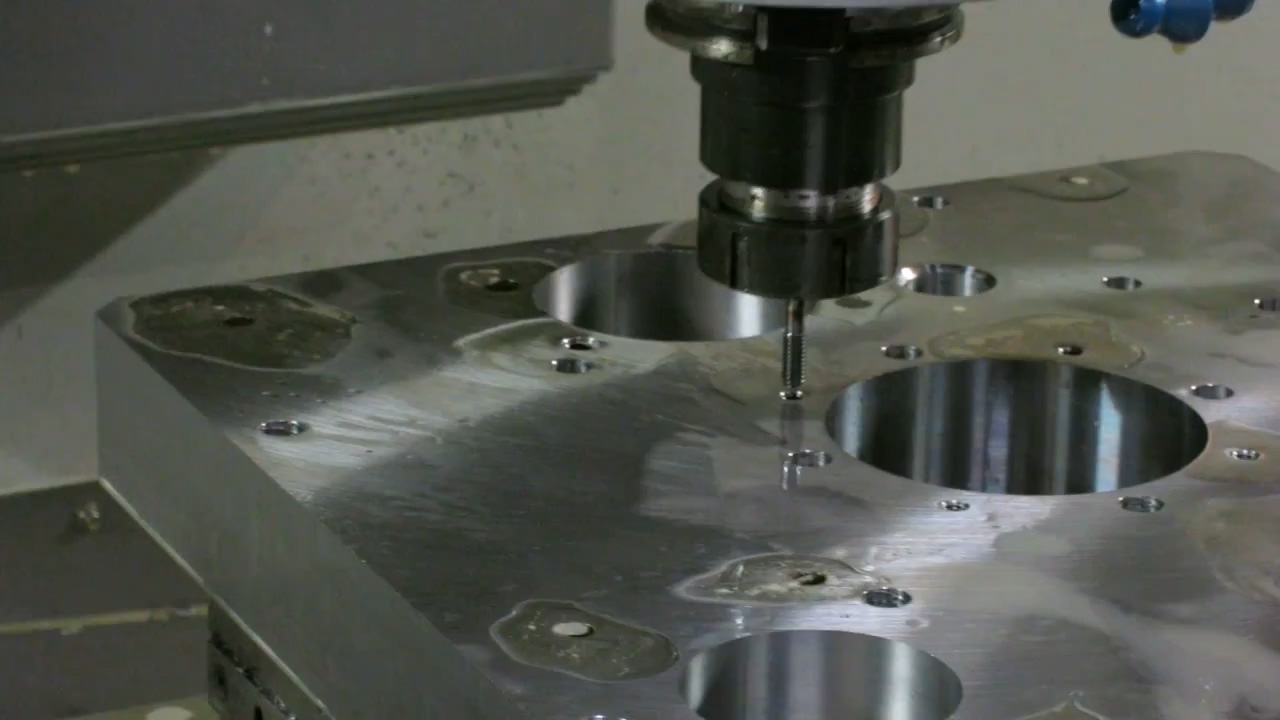
\includegraphics[width=0.5\linewidth,trim=0 0 0 0,clip,angle=0]{image/gangxigongsi.jpg}
	
\end{frame}

\begin{frame}{孔加工方式}
	\begin{columns}
		\column{.05\textwidth}
		\column{.6\textwidth}
		\begin{block}{扩展内容:}
			工厂案例、钻方孔、分割钻孔等
			|\end{block}
		\column{.0\textwidth}
	\end{columns}
	
	\vspace{25pt}
	
	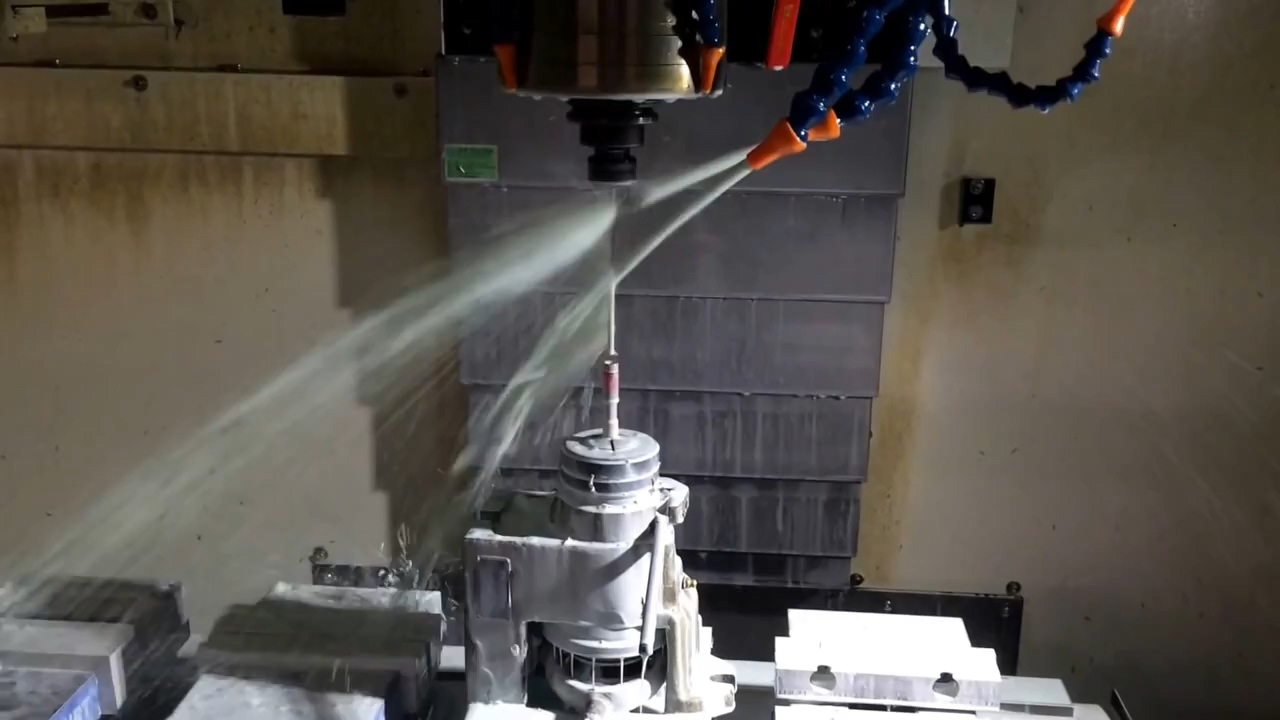
\includegraphics[width=0.5\linewidth,trim=0 0 0 0,clip,angle=0]{image/shengkong.jpg}~
	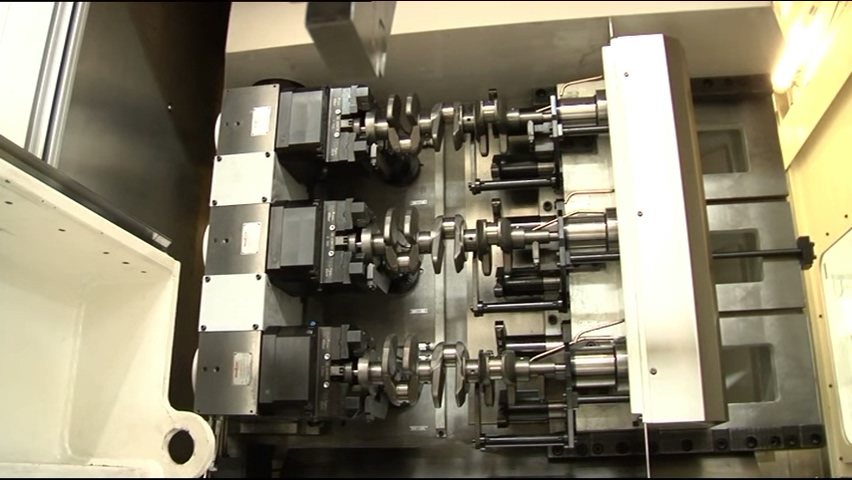
\includegraphics[width=0.5\linewidth,trim=0 0 0 0,clip,angle=0]{image/qubing.jpg}
	
\end{frame}

\begin{frame}{孔加工方式}
	\begin{columns}
		\column{.05\textwidth}
		\column{.6\textwidth}
		\begin{block}{扩展内容:}
			工厂案例、钻方孔、分割钻孔等
			|\end{block}
		\column{.0\textwidth}
	\end{columns}
	
	\vspace{25pt}
	
	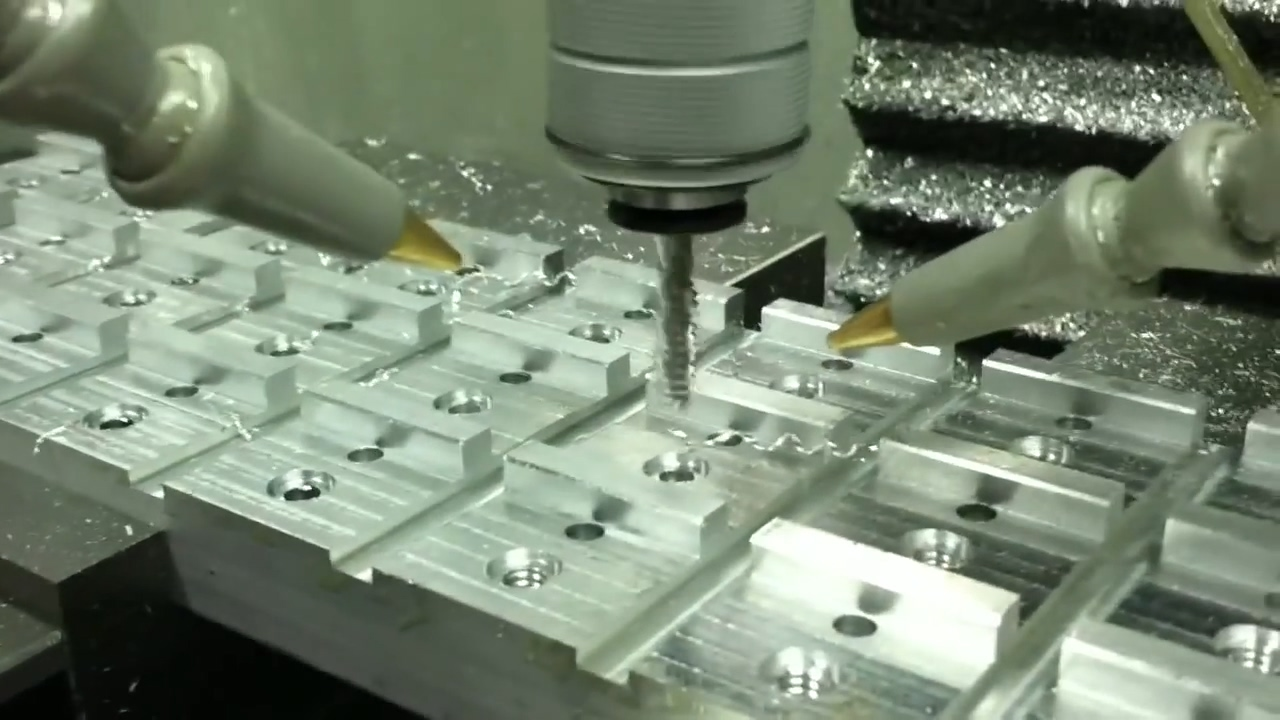
\includegraphics[width=0.5\linewidth,trim=0 0 0 0,clip,angle=0]{image/canpingshili.jpg}~
	
\includegraphics[width=0.5\linewidth,trim=0 0 0 0,clip,angle=0]{image/3}
	
\end{frame}

\begin{frame}{孔加工方式}
	\begin{columns}
		\column{.05\textwidth}
		\column{.6\textwidth}
		\begin{block}{扩展内容:}
			工厂案例、钻方孔、分割钻孔等
			|\end{block}
		\column{.0\textwidth}
	\end{columns}
	
	\vspace{25pt}
	
	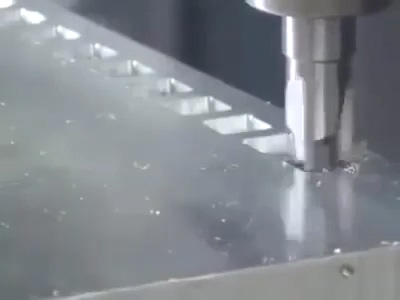
\includegraphics[width=0.5\linewidth,trim=0 0 0 0,clip,angle=0]{image/zuanfangkong.jpg}~
	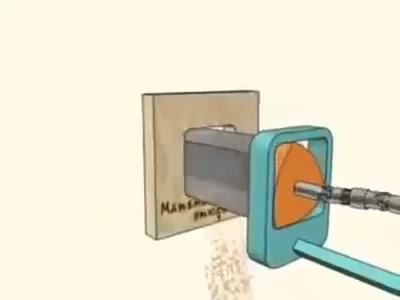
\includegraphics[width=0.5\linewidth,trim=0 0 0 0,clip,angle=0]{image/zuanfangkongyuanli.jpg}
	
\end{frame}

\begin{frame}{孔加工方式}
	\begin{columns}
		\column{.05\textwidth}
		\column{.6\textwidth}
		\begin{block}{扩展内容:}
			工厂案例、钻方孔、分割钻孔等
			|\end{block}
		\column{.0\textwidth}
	\end{columns}
	
	\vspace{25pt}
	
	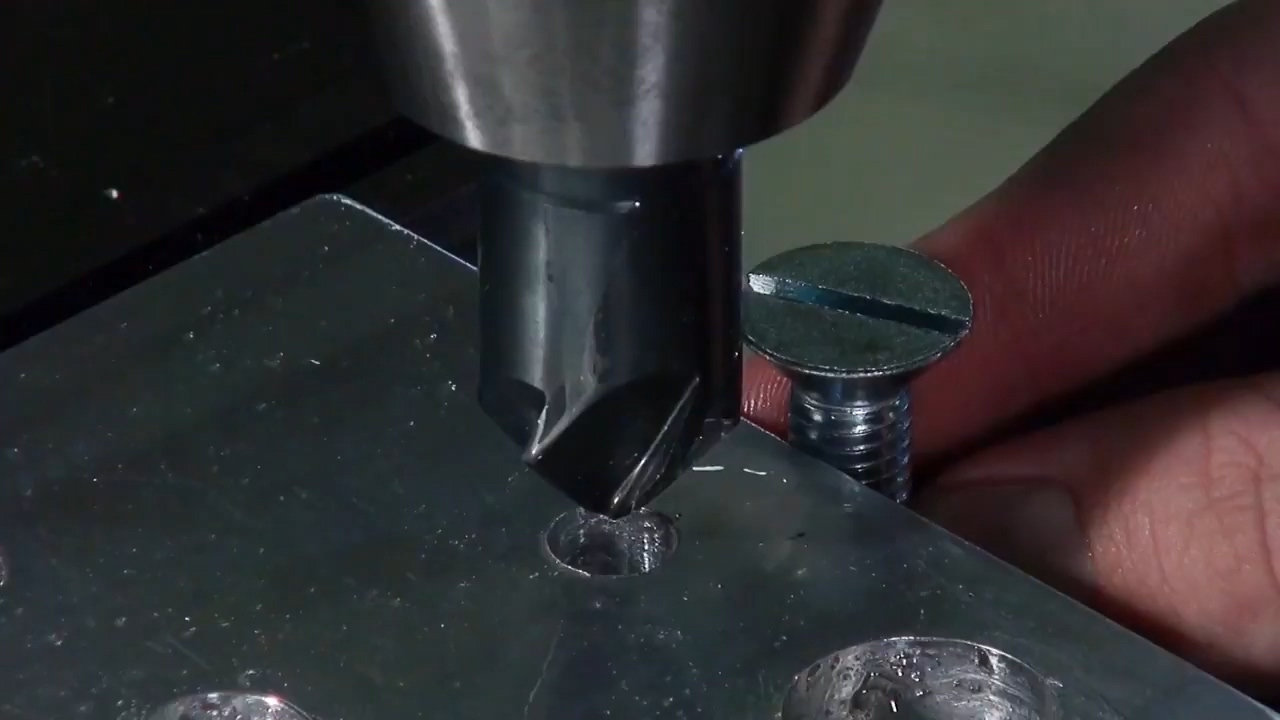
\includegraphics[width=0.3\linewidth,trim=0 0 0 0,clip,angle=0]{image/zhuikong.jpg}~
	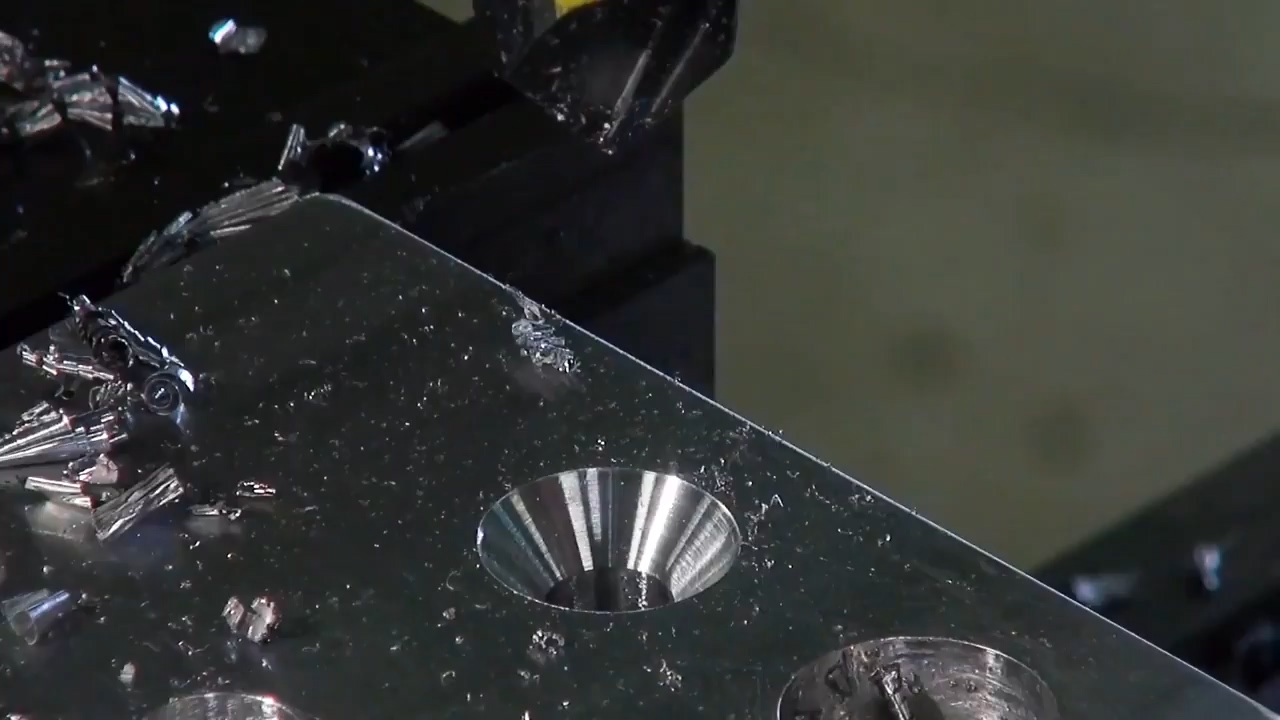
\includegraphics[width=0.3\linewidth,trim=0 0 0 0,clip,angle=0]{image/zhuimian.jpg}`
	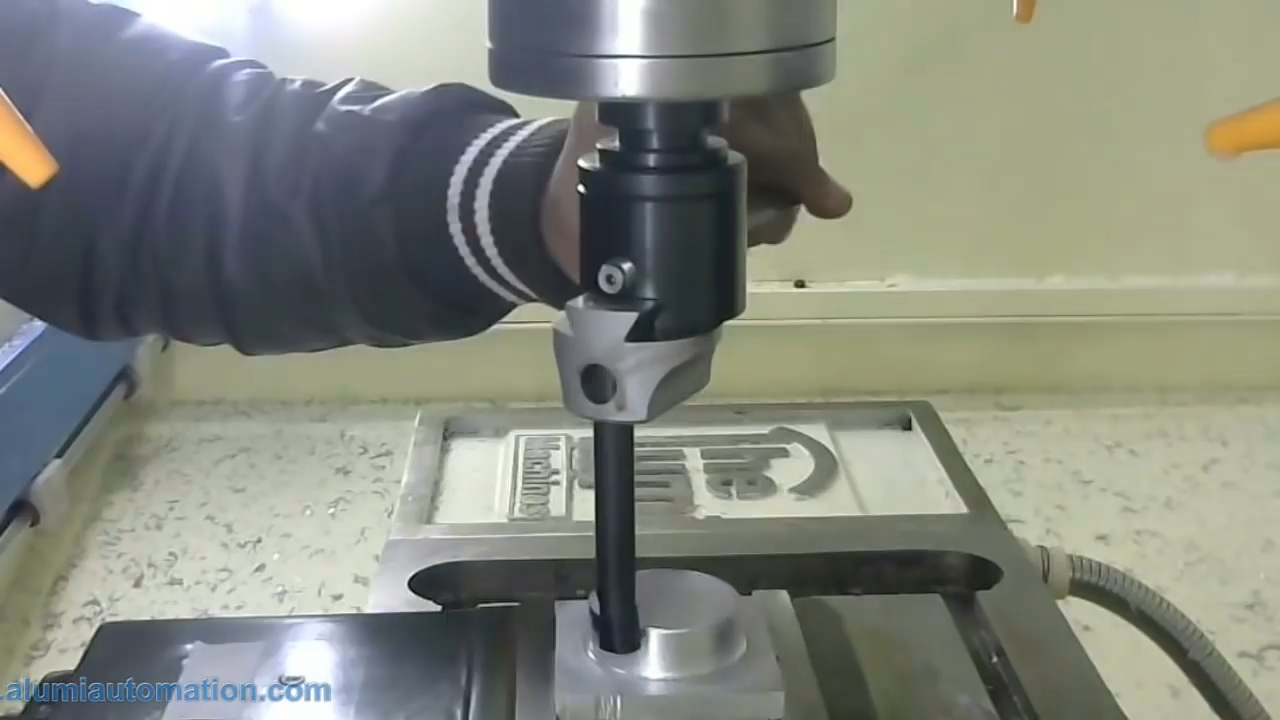
\includegraphics[width=0.3\linewidth,trim=0 0 0 0,clip,angle=0]{image/tangwaixing.jpg}
	
\end{frame}

\begin{frame}{孔加工方式}
	\begin{columns}
		\column{.05\textwidth}
		\column{.6\textwidth}
		\begin{block}{扩展内容:}
			工厂案例、钻方孔、分割钻孔等
			|\end{block}
		\column{.0\textwidth}
	\end{columns}
	
	\vspace{25pt}
	
	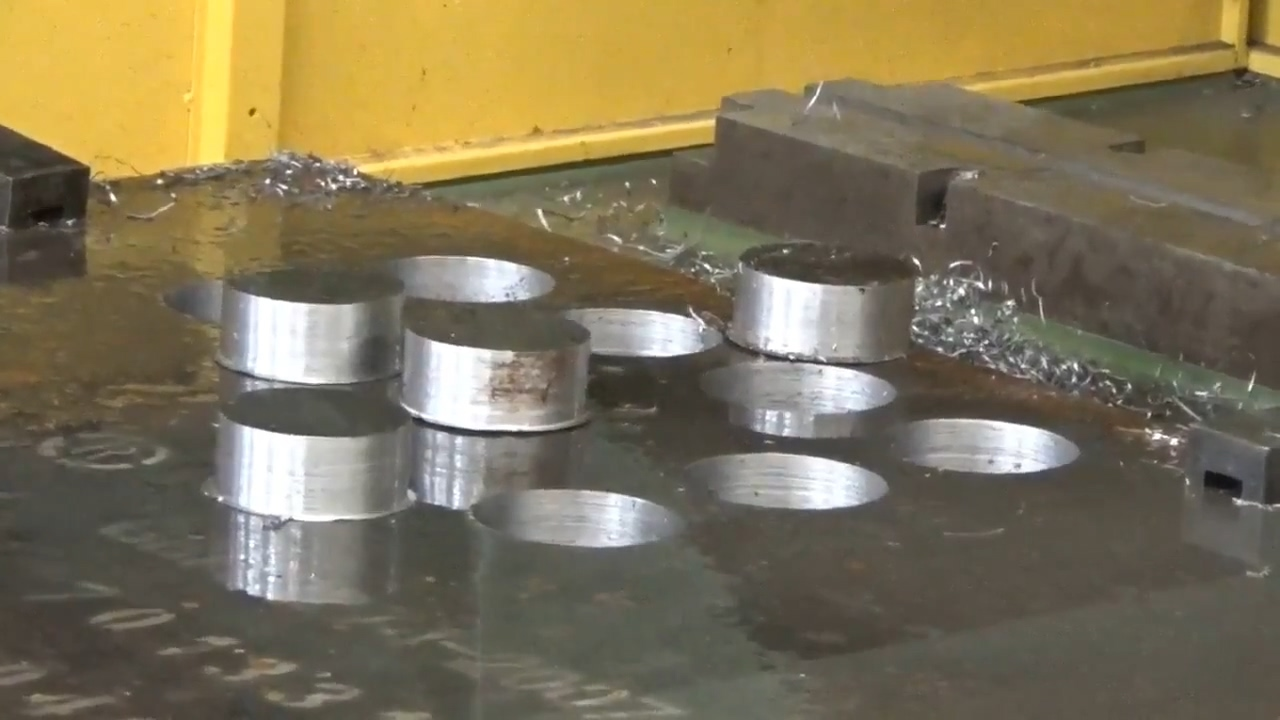
\includegraphics[width=0.3\linewidth,trim=0 0 0 0,clip,angle=0]{image/fengezuankong.jpg}~
	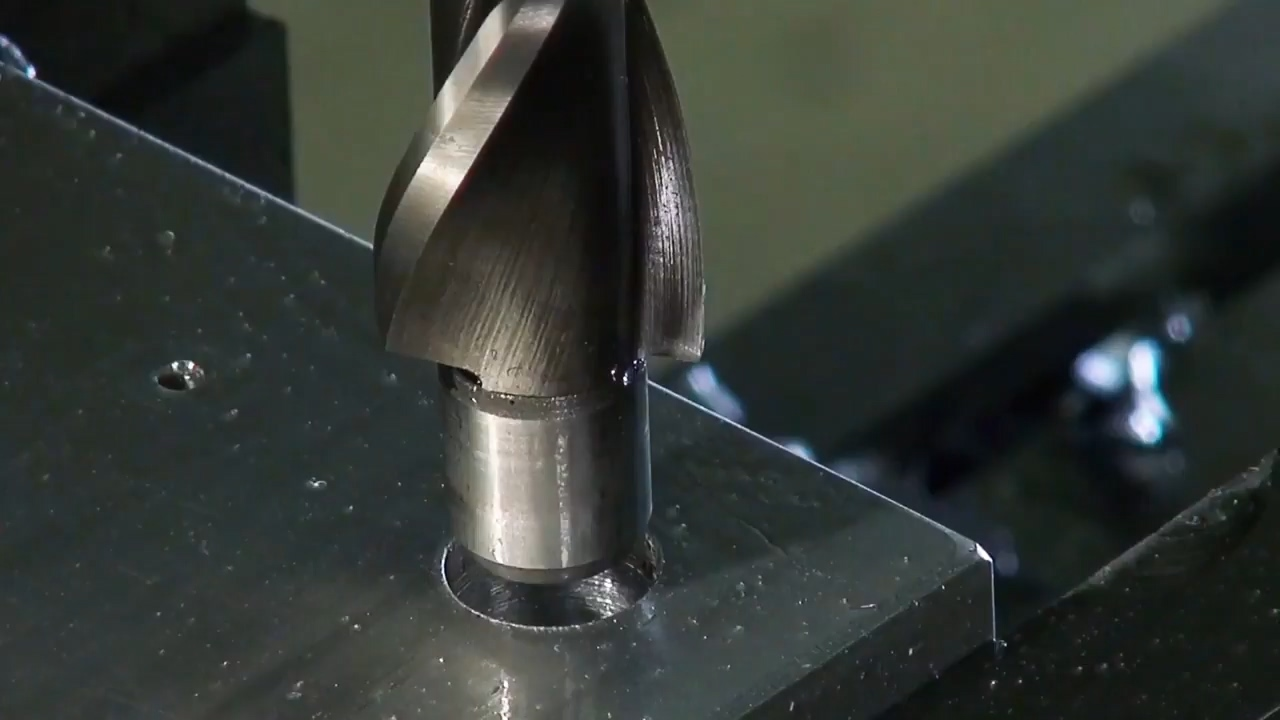
\includegraphics[width=0.3\linewidth,trim=0 0 0 0,clip,angle=0]{image/fukong.jpg}`
	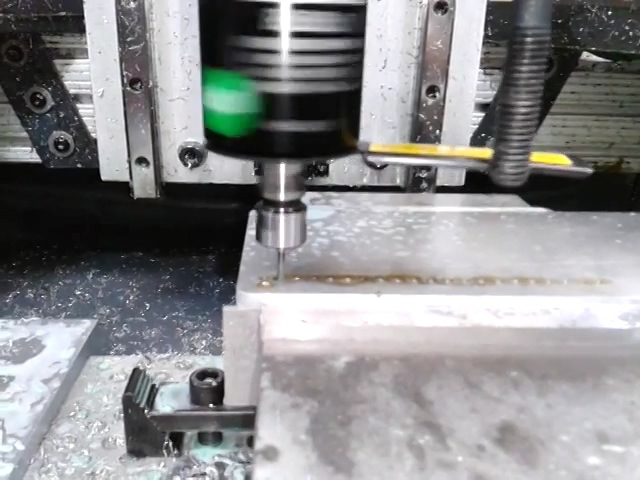
\includegraphics[width=0.3\linewidth,trim=0 0 0 0,clip,angle=0]{image/rouxinggongsi.jpg}
	
\end{frame}

\begin{frame}{孔加工方式}
	\begin{columns}
		\column{.05\textwidth}
		\column{.6\textwidth}
		\begin{block}{工厂现场:}
			6S要求讲解,别人的习惯。
			|\end{block}
		\column{.0\textwidth}
	\end{columns}
	
	\vspace{25pt}
	
	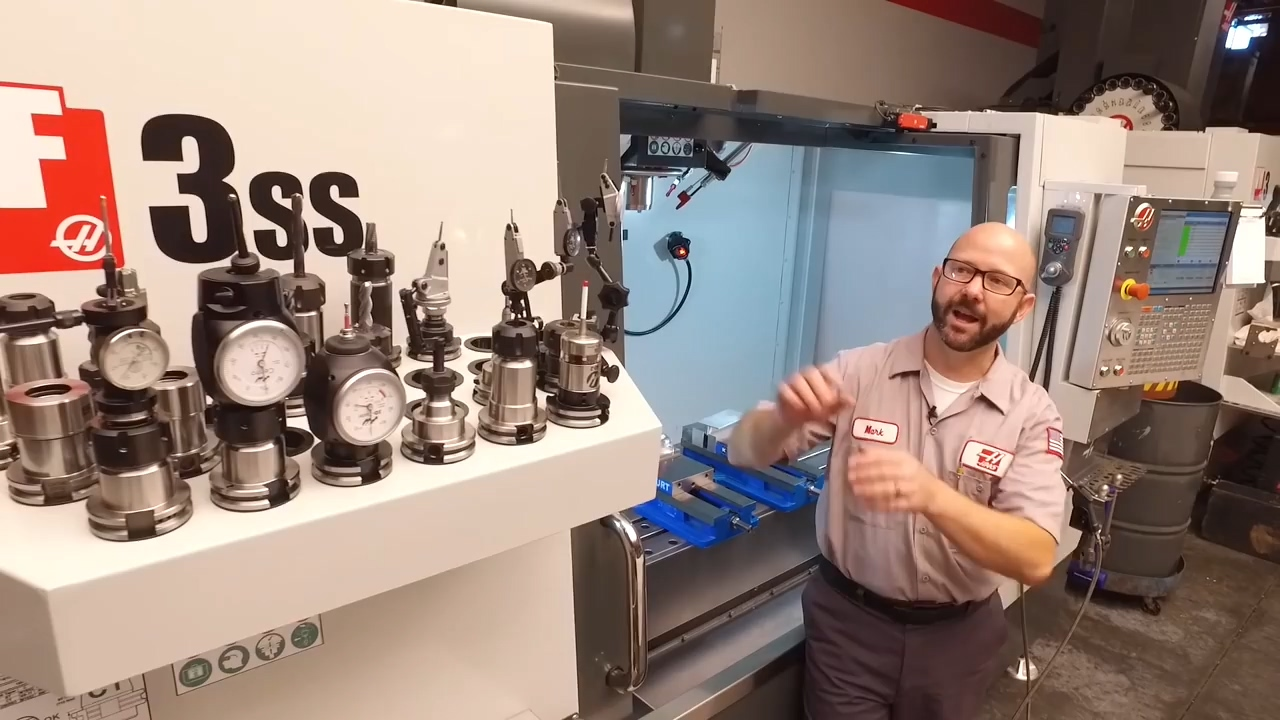
\includegraphics[width=0.6\linewidth,trim=0 0 0 0,clip,angle=0]{image/gongzuohuaijing.jpg}~
	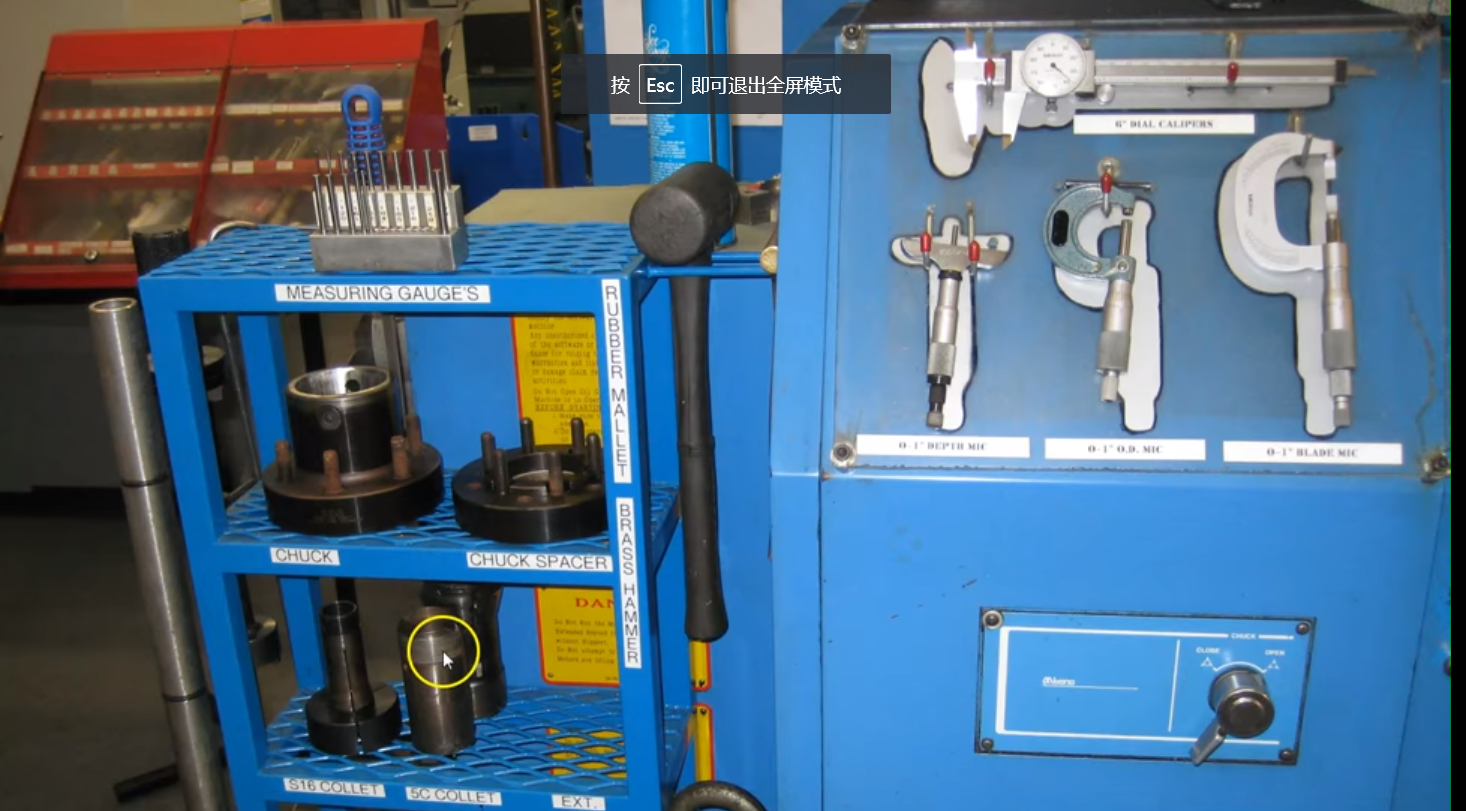
\includegraphics[width=0.4\linewidth,trim=0 0 0 0,clip,angle=0]{image/6s}
	
\end{frame}

\begin{frame}{孔加工方式}
	\begin{columns}
		\column{.05\textwidth}
		\column{.6\textwidth}
		\begin{block}{工厂现场:}
			6S要求讲解,别人的习惯。
			|\end{block}
		\column{.0\textwidth}
	\end{columns}
	
	\vspace{25pt}
	
	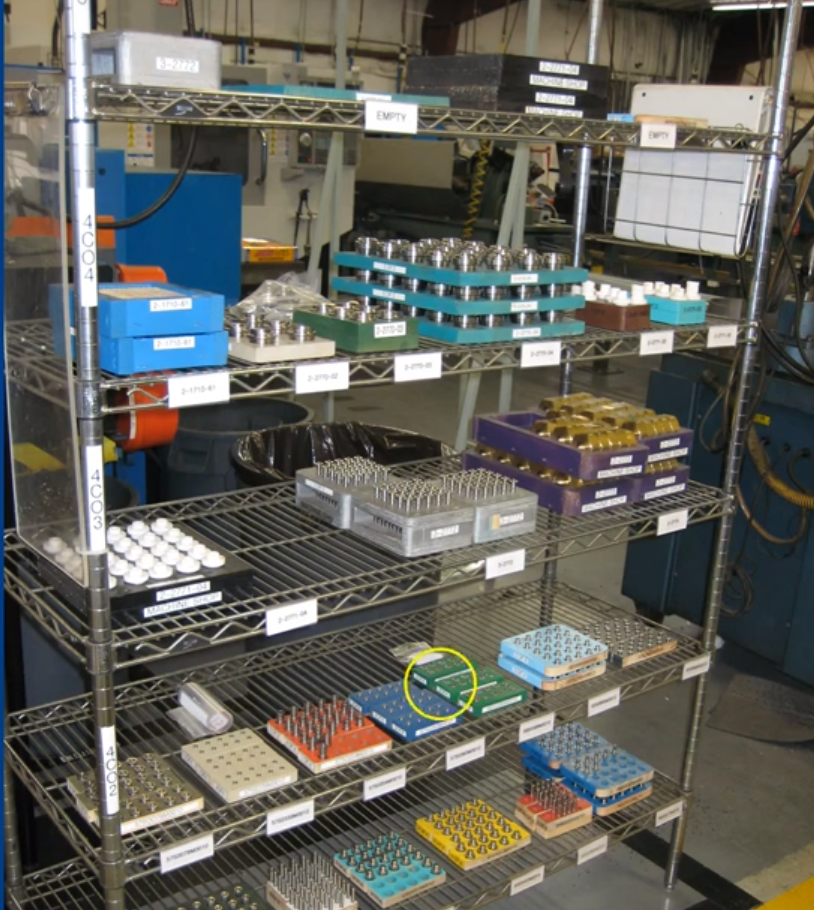
\includegraphics[width=.3\linewidth,trim=0 0 0  0,clip,angle=0]{image/6s2}~
	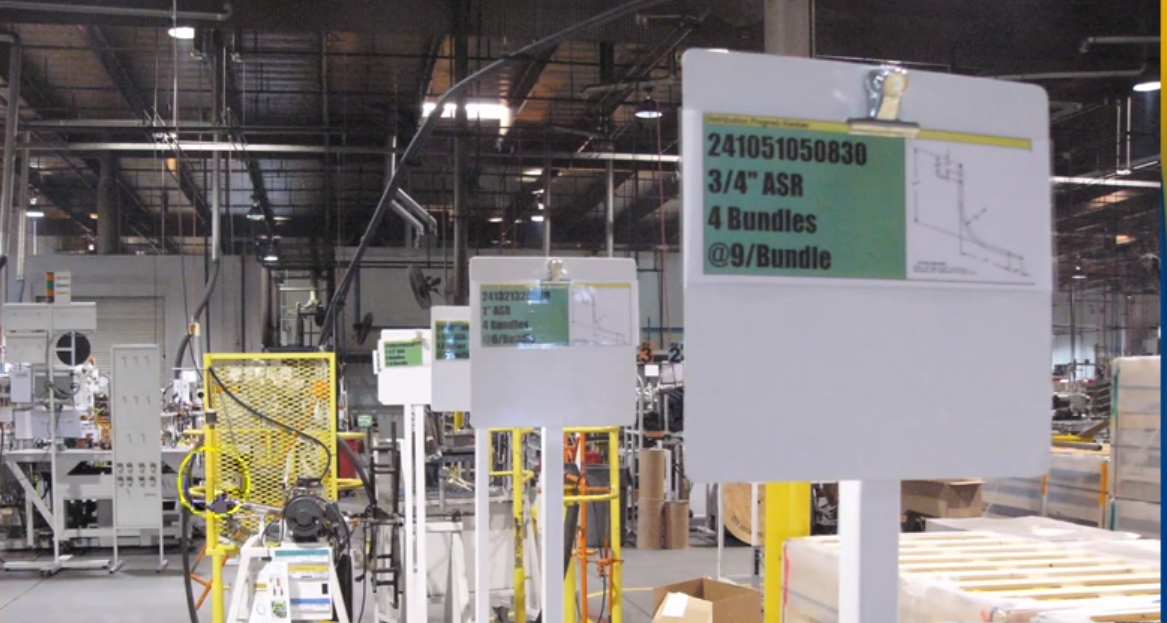
\includegraphics[width=0.6\linewidth,trim=0 0 0 0,clip,angle=0]{image/6s1}
	
\end{frame}


\begin{frame}{孔加工方式}
	\begin{columns}
		\column{.05\textwidth}
		\column{.6\textwidth}
		\begin{block}{安全意识:}
			有安全隐患的视频。
			|\end{block}
		\column{.0\textwidth}
	\end{columns}
	
	\vspace{25pt}
	
	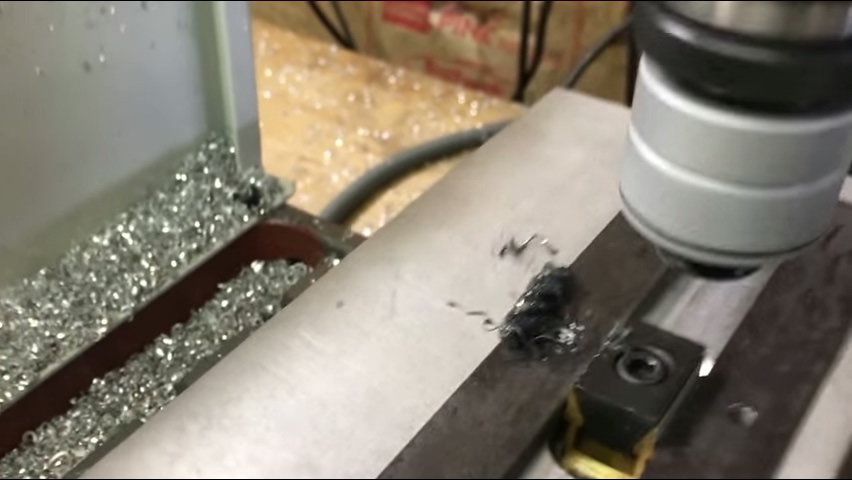
\includegraphics[width=.5\linewidth,trim=0 0 0  0,clip,angle=0]{image/duandao.jpg}~
	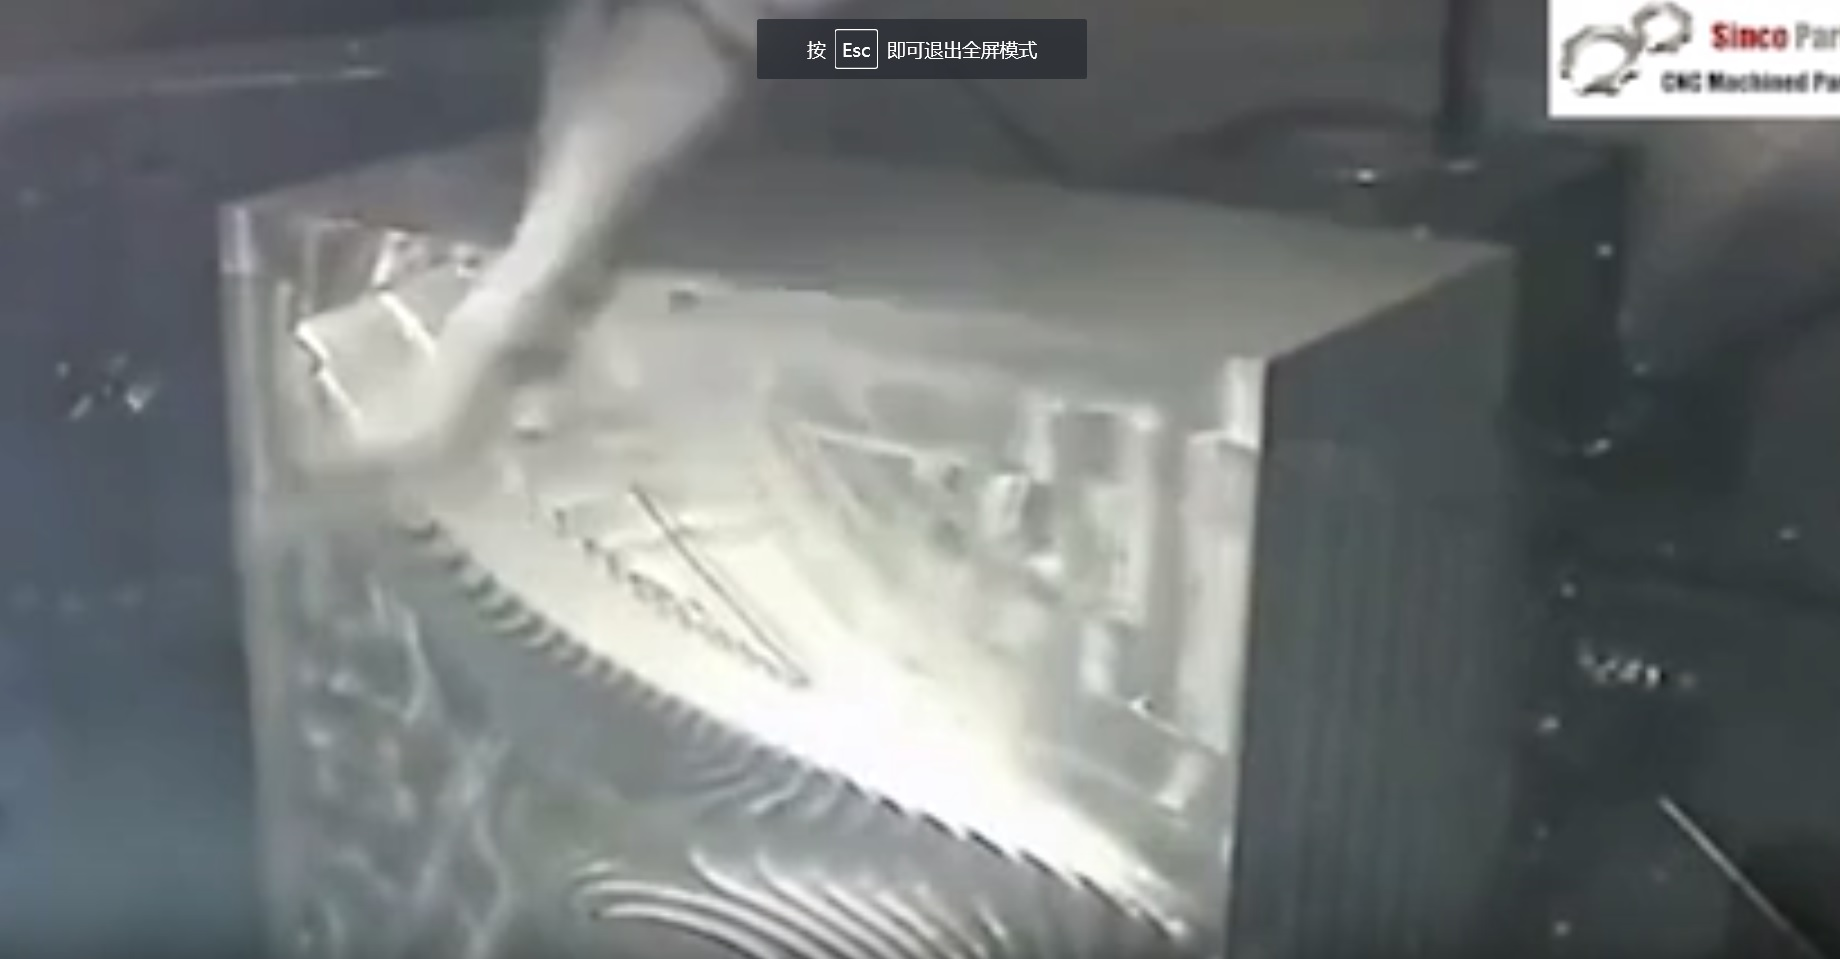
\includegraphics[width=0.5\linewidth,trim=0 0 0 0,clip,angle=0]{image/anquandadao.jpg}
	
\end{frame}

\begin{frame}{孔加工方式}
	\begin{columns}
		\column{.05\textwidth}
		\column{.6\textwidth}
		\begin{block}{安全意识:}
			有安全隐患的视频。
			|\end{block}
		\column{.0\textwidth}
	\end{columns}
	
	\vspace{25pt}
	
	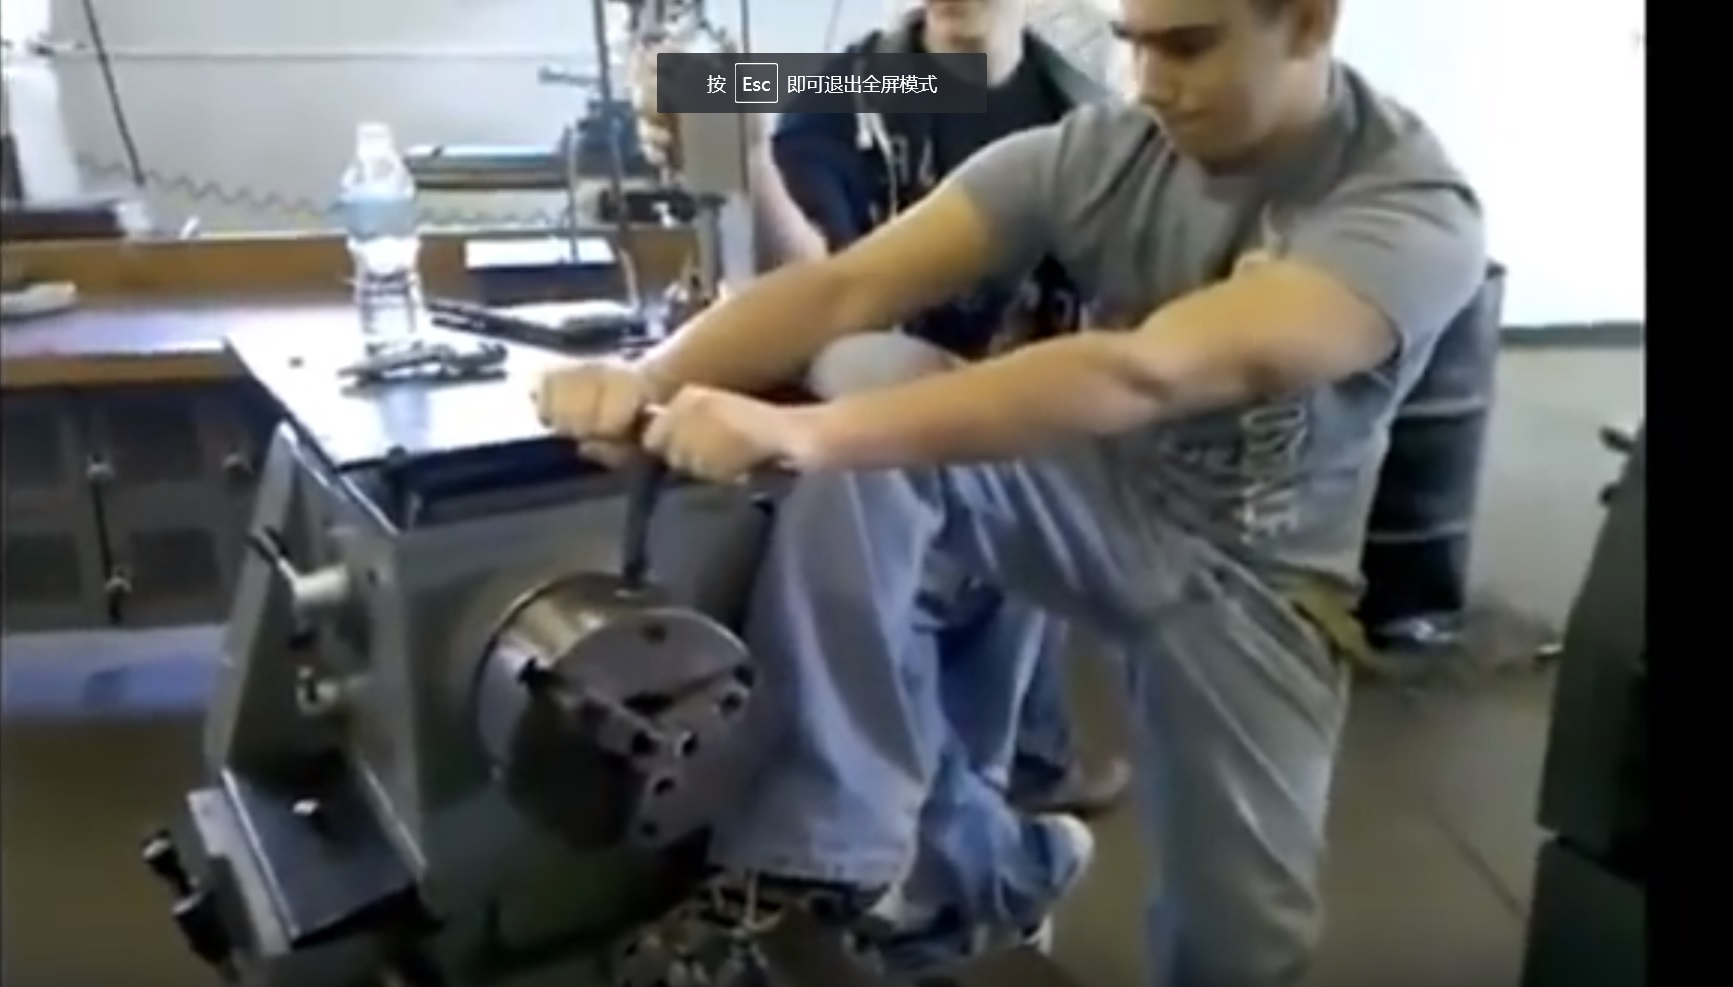
\includegraphics[width=.5\linewidth,trim=0 0 0  0,clip,angle=0]{image/anquan1.jpg}~
	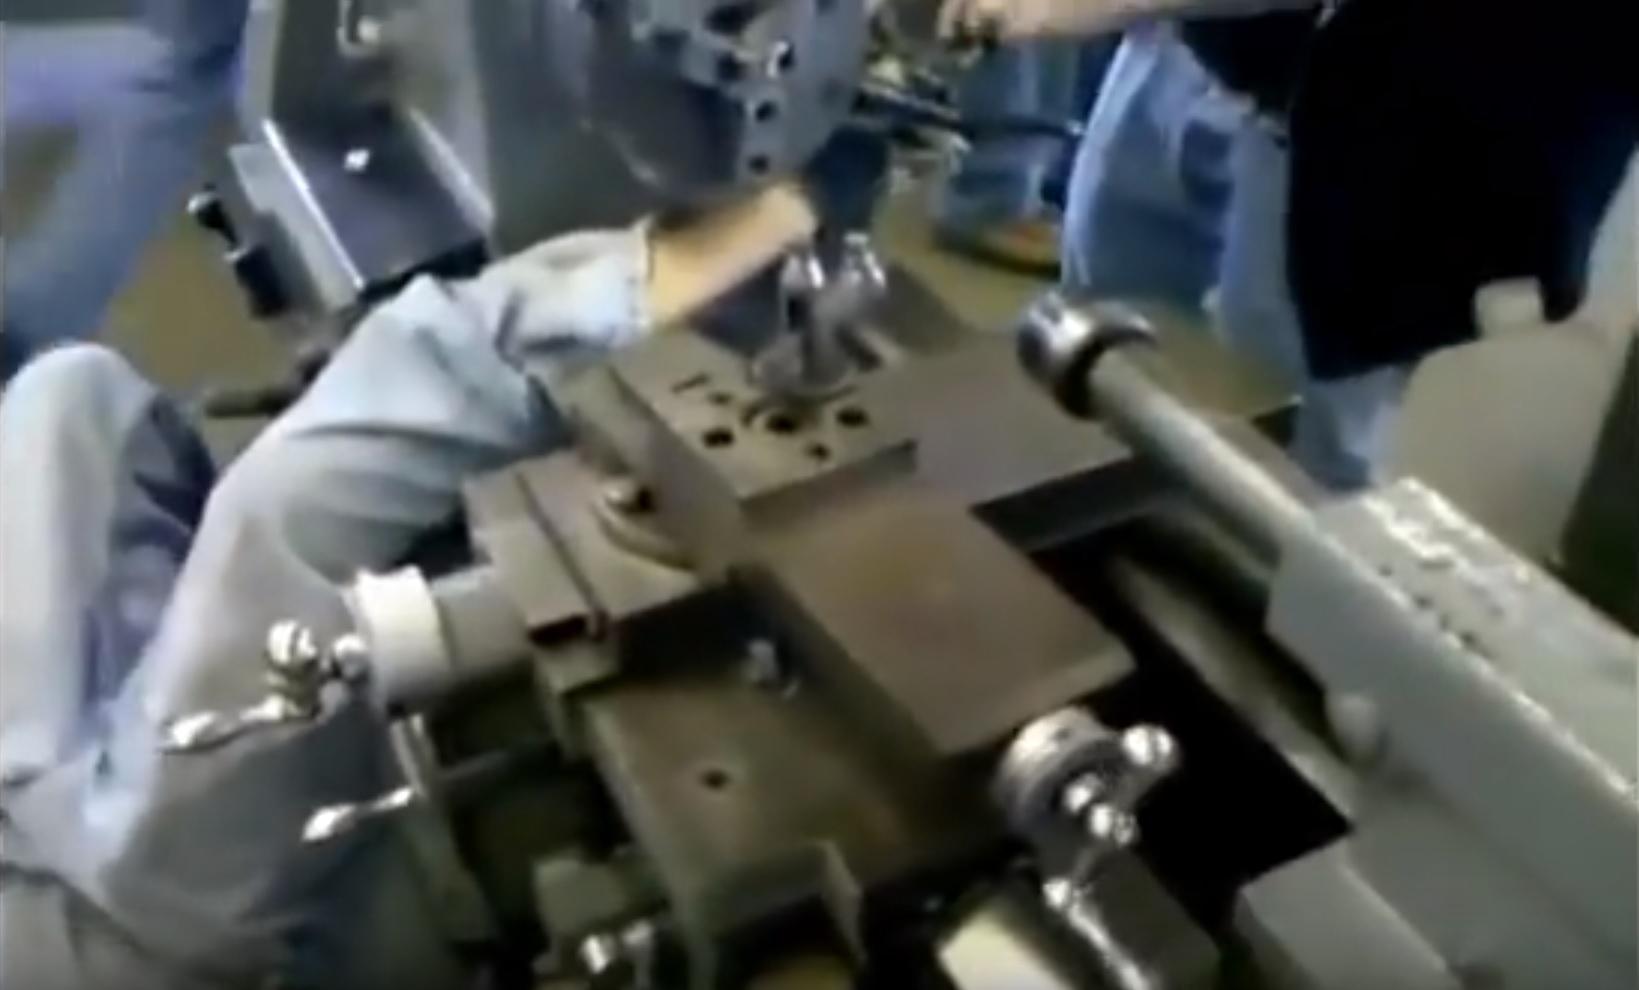
\includegraphics[width=0.5\linewidth,trim=0 0 0 0,clip,angle=0]{image/anquan2.jpg}
	
\end{frame}

\begin{frame}{孔加工方式}
	\begin{columns}
		\column{.05\textwidth}
		\column{.6\textwidth}
		\begin{block}{安全意识:}
			有安全隐患的视频。
			|\end{block}
		\column{.0\textwidth}
	\end{columns}
	
	\vspace{25pt}
	
	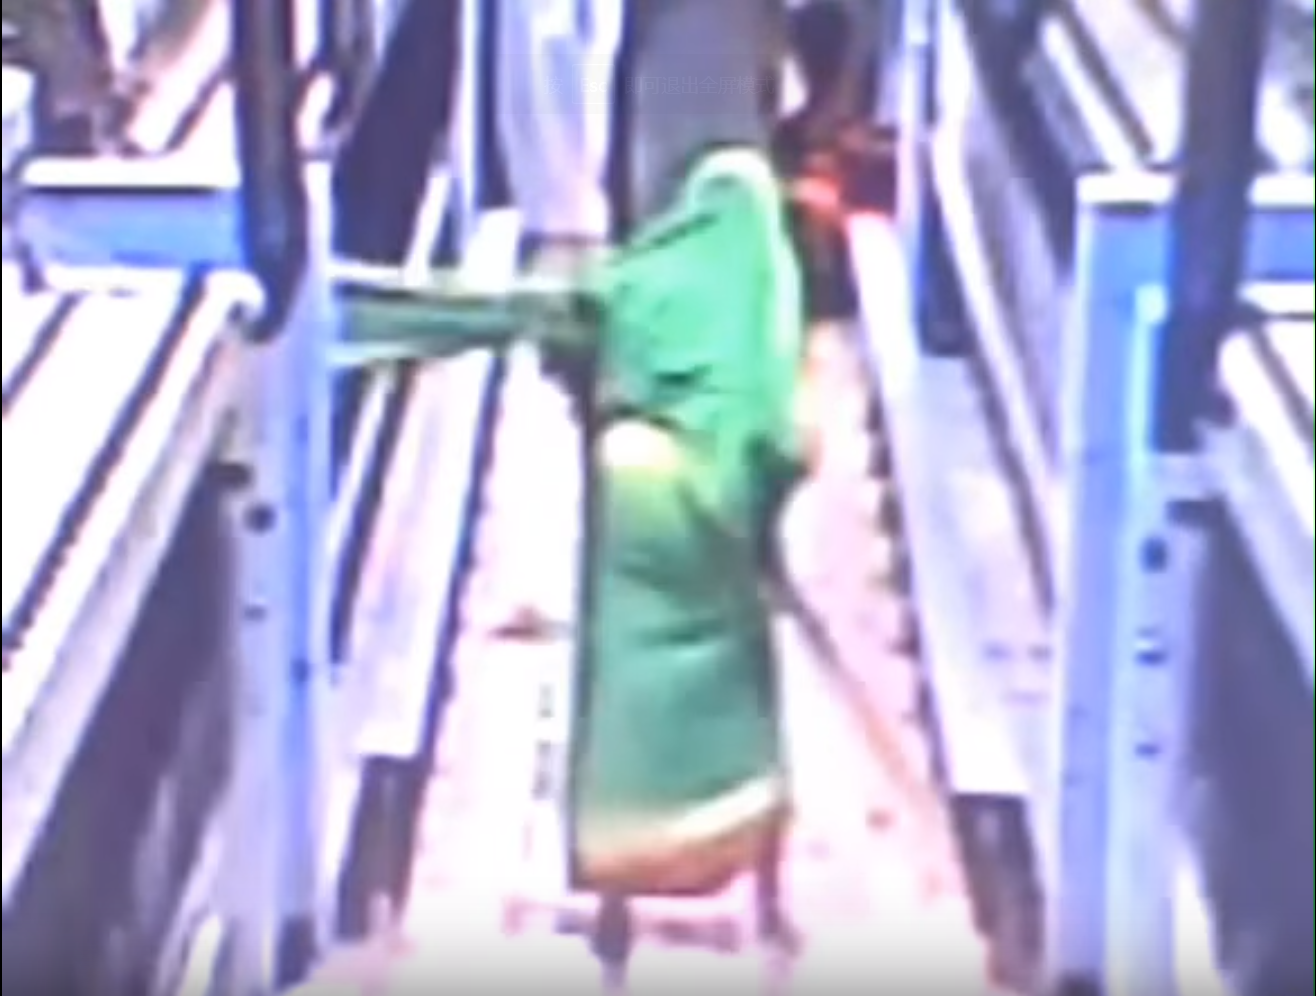
\includegraphics[width=.5\linewidth,trim=0 0 0  0,clip,angle=0]{image/anquan3.png}~
	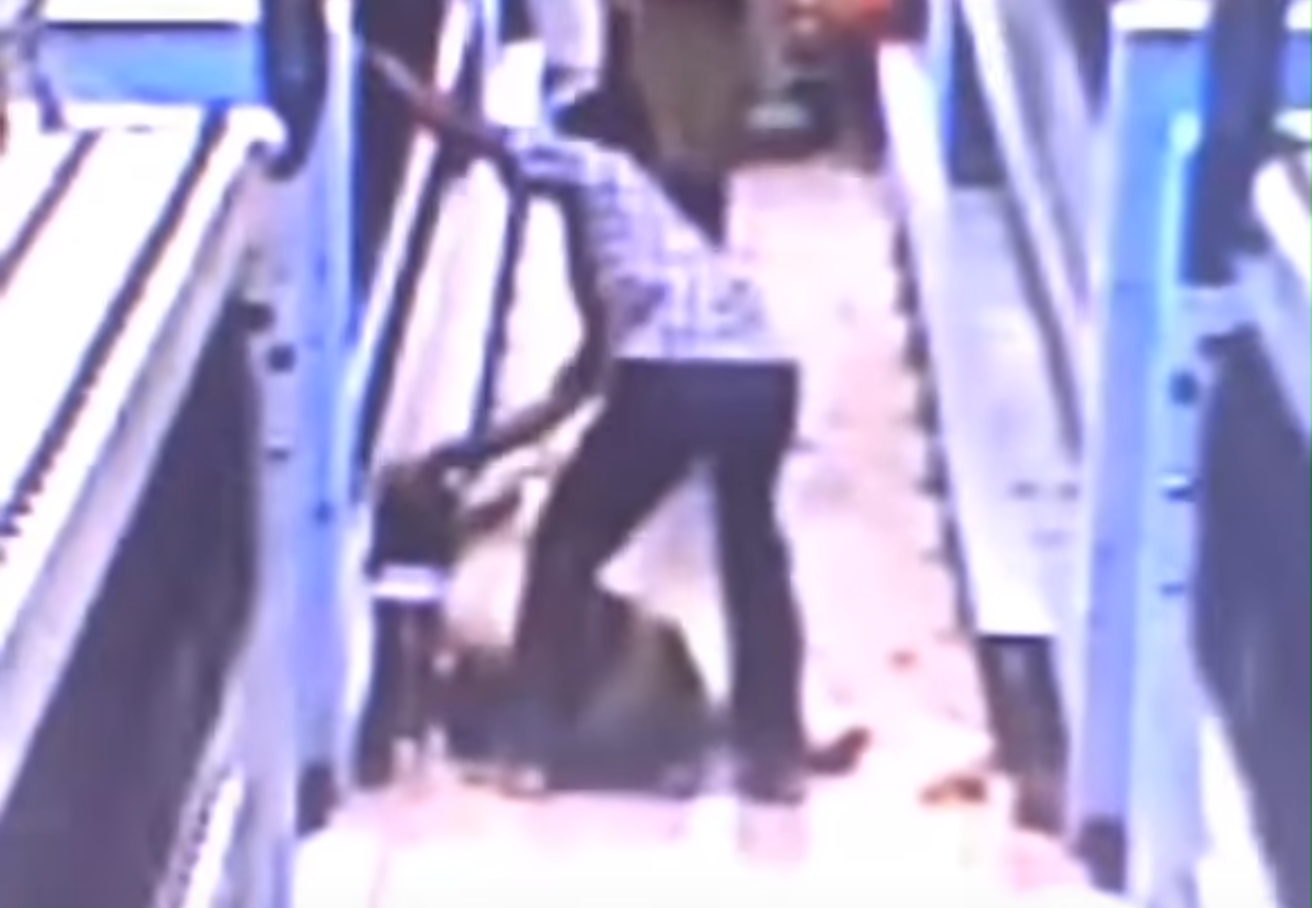
\includegraphics[width=0.5\linewidth,trim=0 0 0 0,clip,angle=0]{image/anquan4.png}
	
\end{frame}

\begin{frame}{孔加工方式}
	\begin{columns}
		\column{.05\textwidth}
		\column{.6\textwidth}
		\begin{block}{安全意识:}
			有安全隐患的视频。
			|\end{block}
		\column{.0\textwidth}
	\end{columns}
	
	\vspace{25pt}
	
	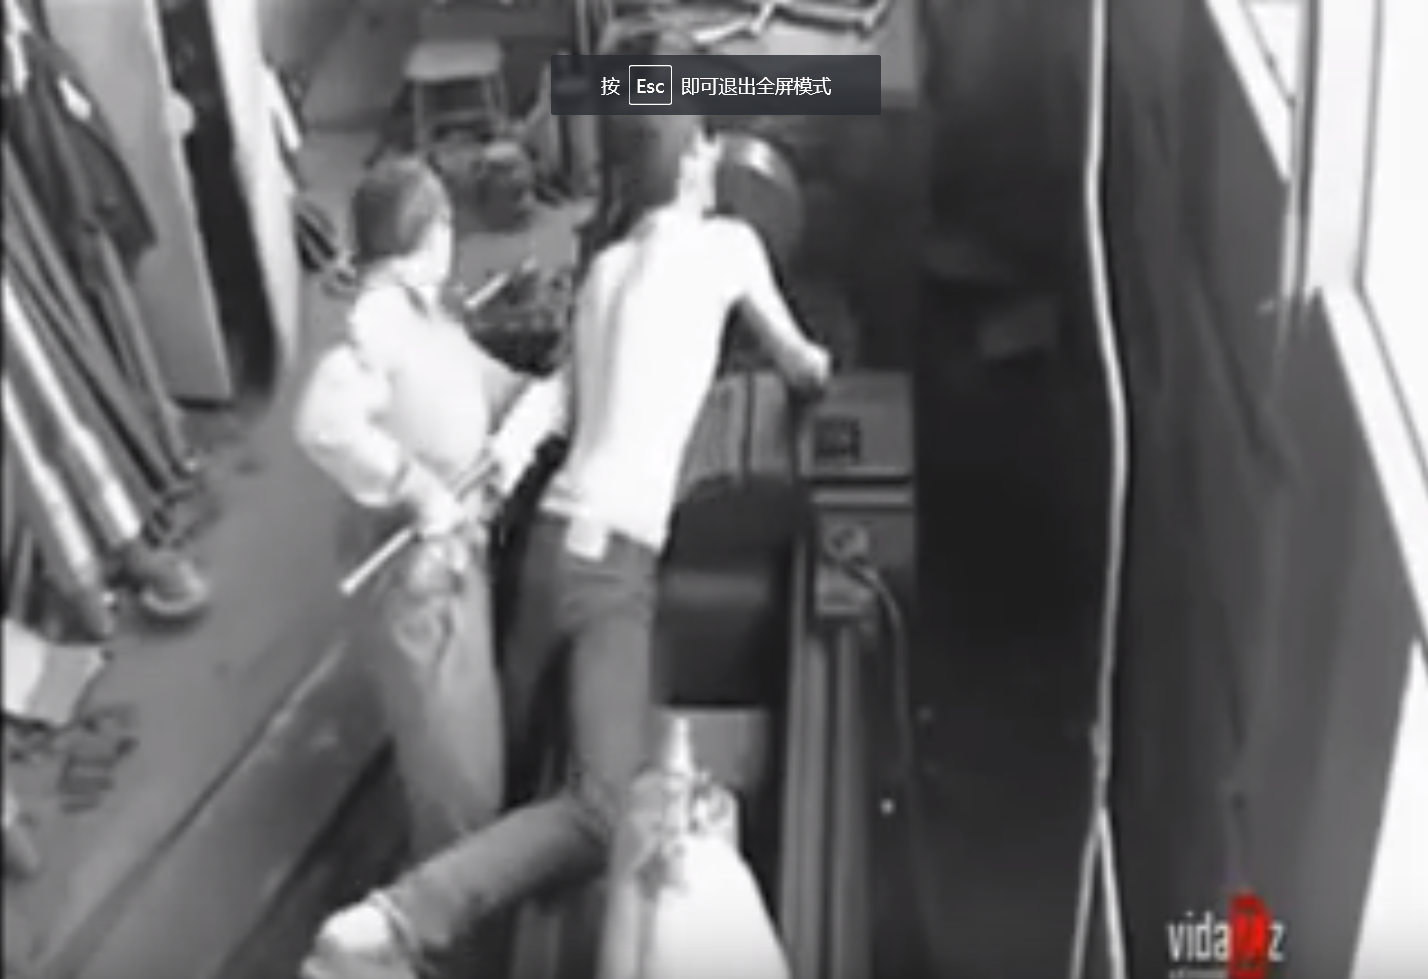
\includegraphics[width=.3\linewidth,trim=0 0 0  0,clip,angle=0]{image/anquan5.png}~
	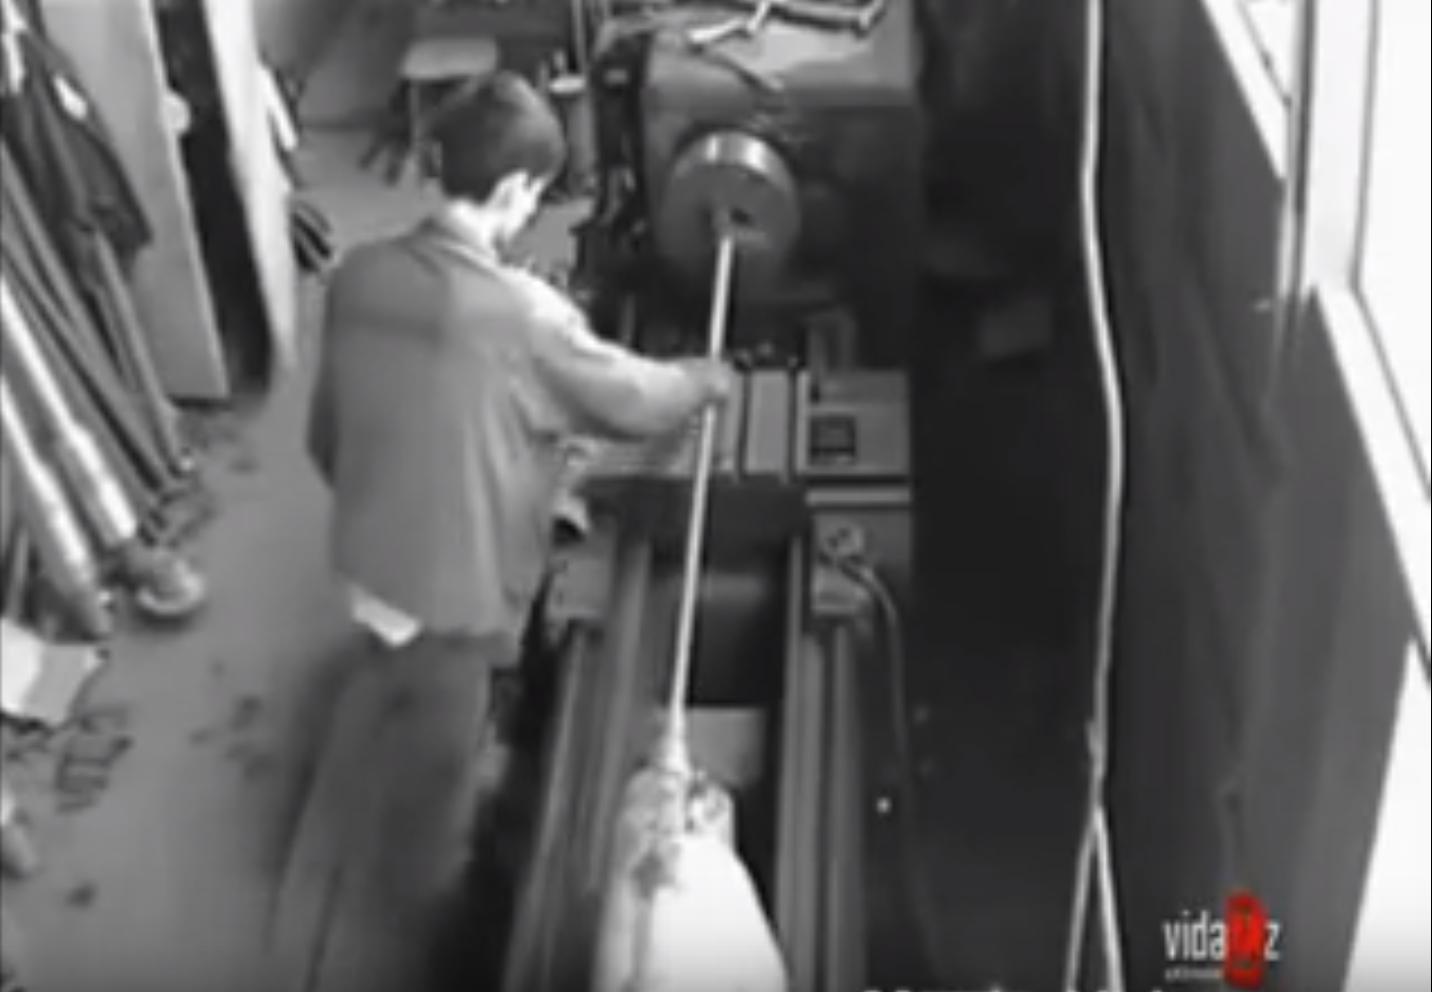
\includegraphics[width=0.3\linewidth,trim=0 0 0 0,clip,angle=0]{image/anquan6.png}~
	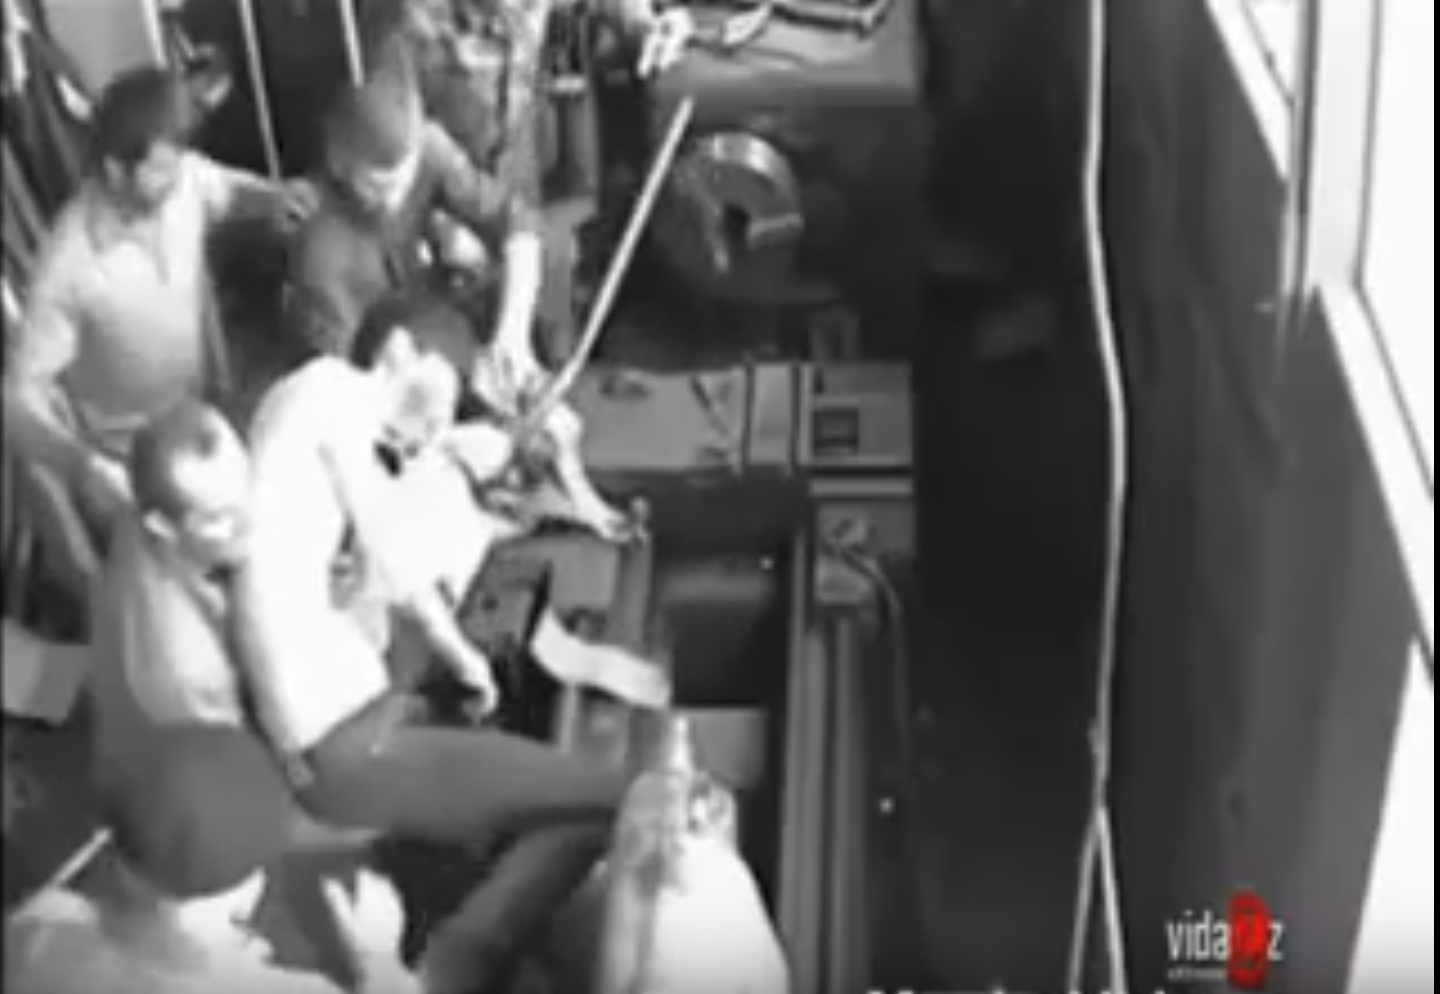
\includegraphics[width=0.3\linewidth,trim=0 0 0 0,clip,angle=0]{image/anquan7.png}	
\end{frame}

\begin{frame}{孔加工刀具}
	\begin{columns}
		\column{0\textwidth}
		\column{\textwidth}
		
		实物展示:中心钻、麻花钻、铰刀、镗刀、丝锥

		
		\column{0\textwidth}
	\end{columns}


\includegraphics[width=.5\linewidth,trim=0 0 0  0,clip,angle=0]{image/4}~
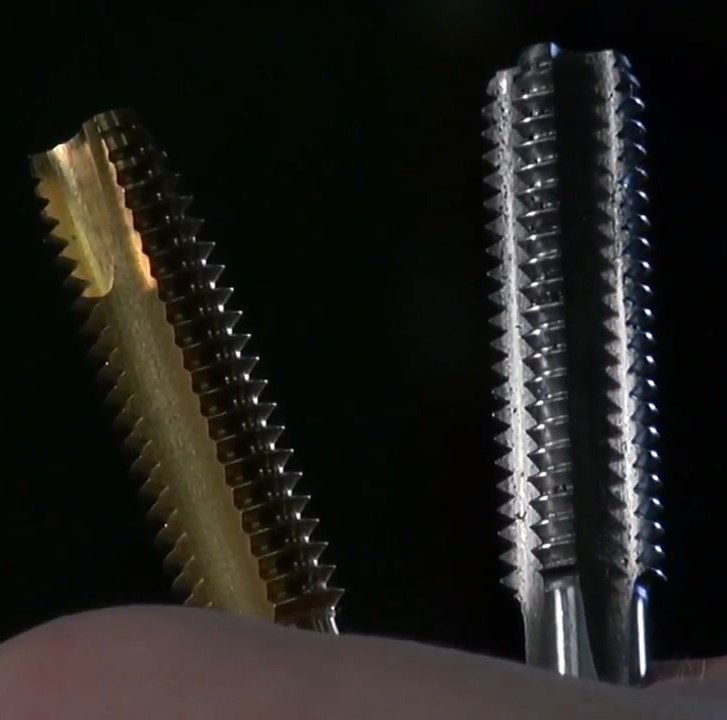
\includegraphics[width=0.5\linewidth,trim=0 0 0 0,clip,angle=0]{image/sizui.jpg}~
\end{frame}

\begin{frame}{孔加工刀具}
		
			
提供关键字,学生上网淘宝查。

BT40镗刀柄、钻夹刀柄、柔性刀柄

价格与型号。

\centering
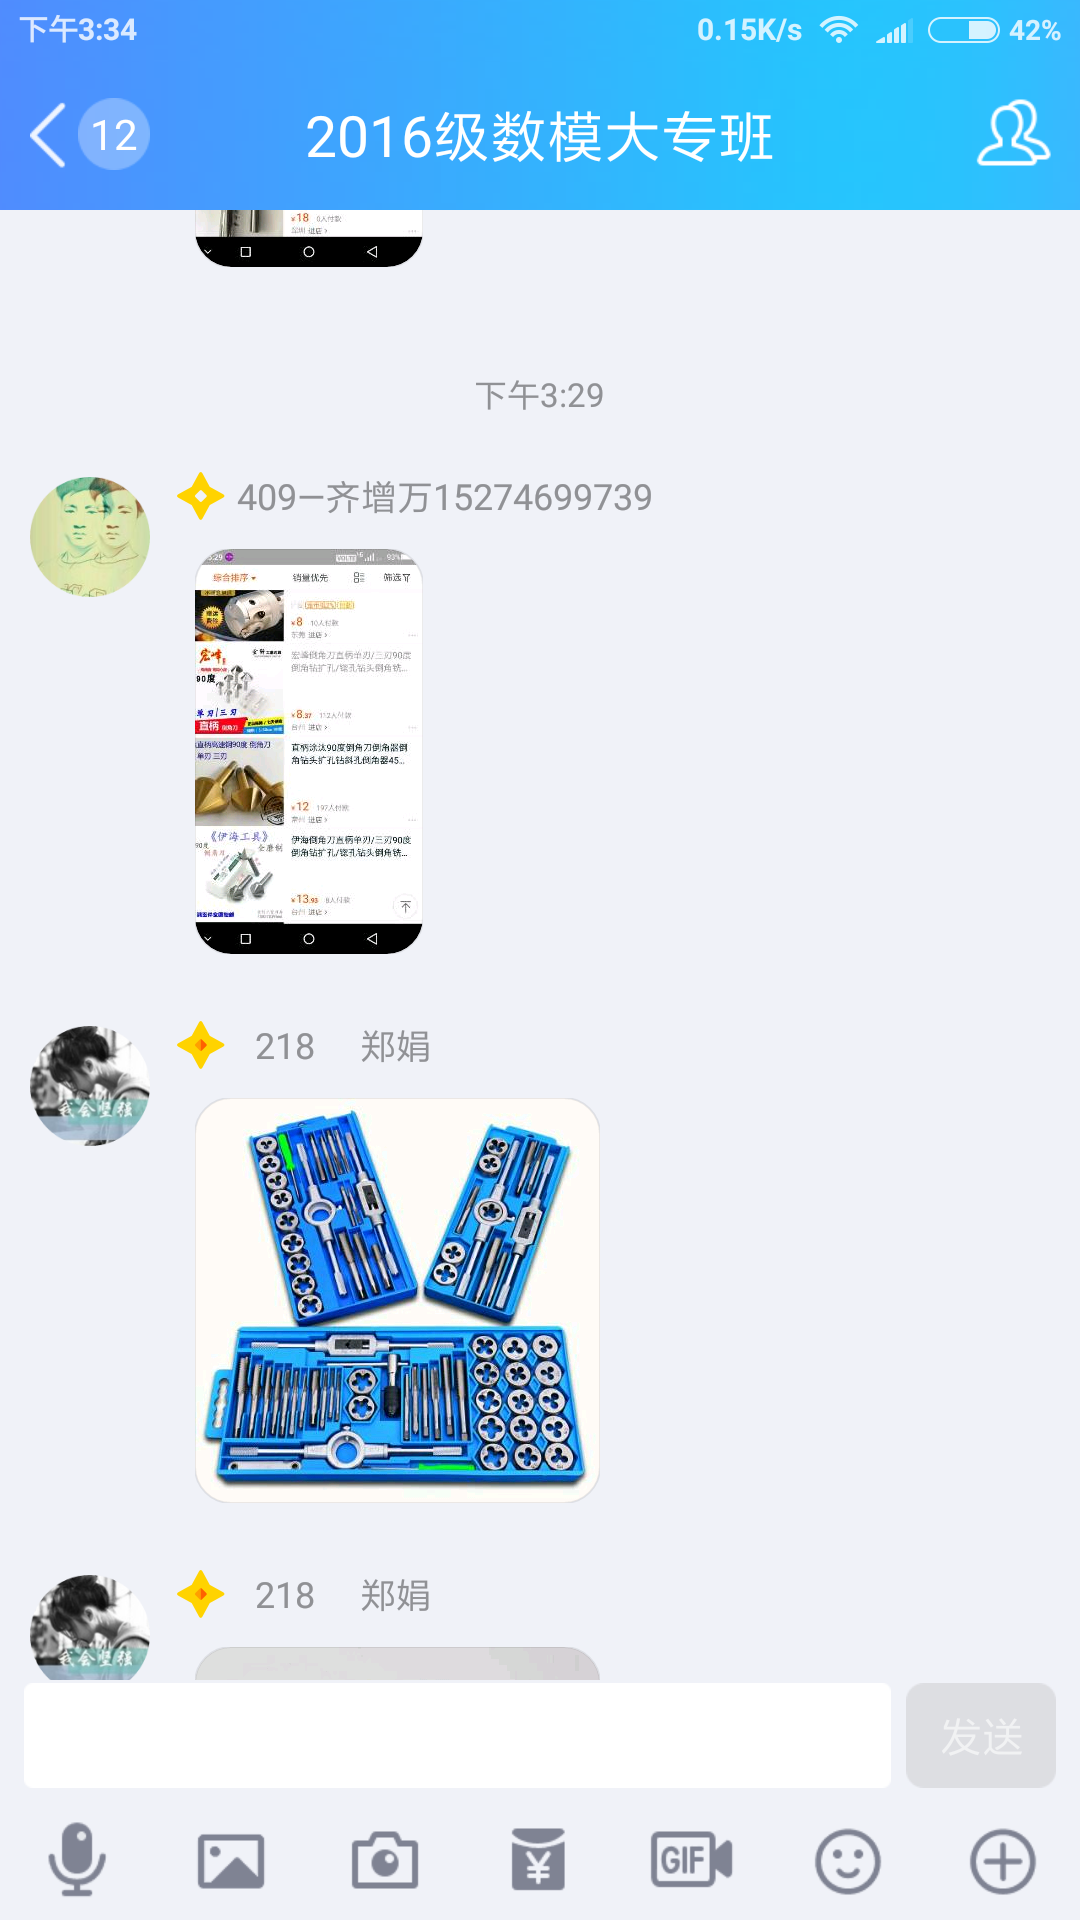
\includegraphics[width=.2\linewidth,trim=0 0 0  0,clip,angle=0]{image/21}~
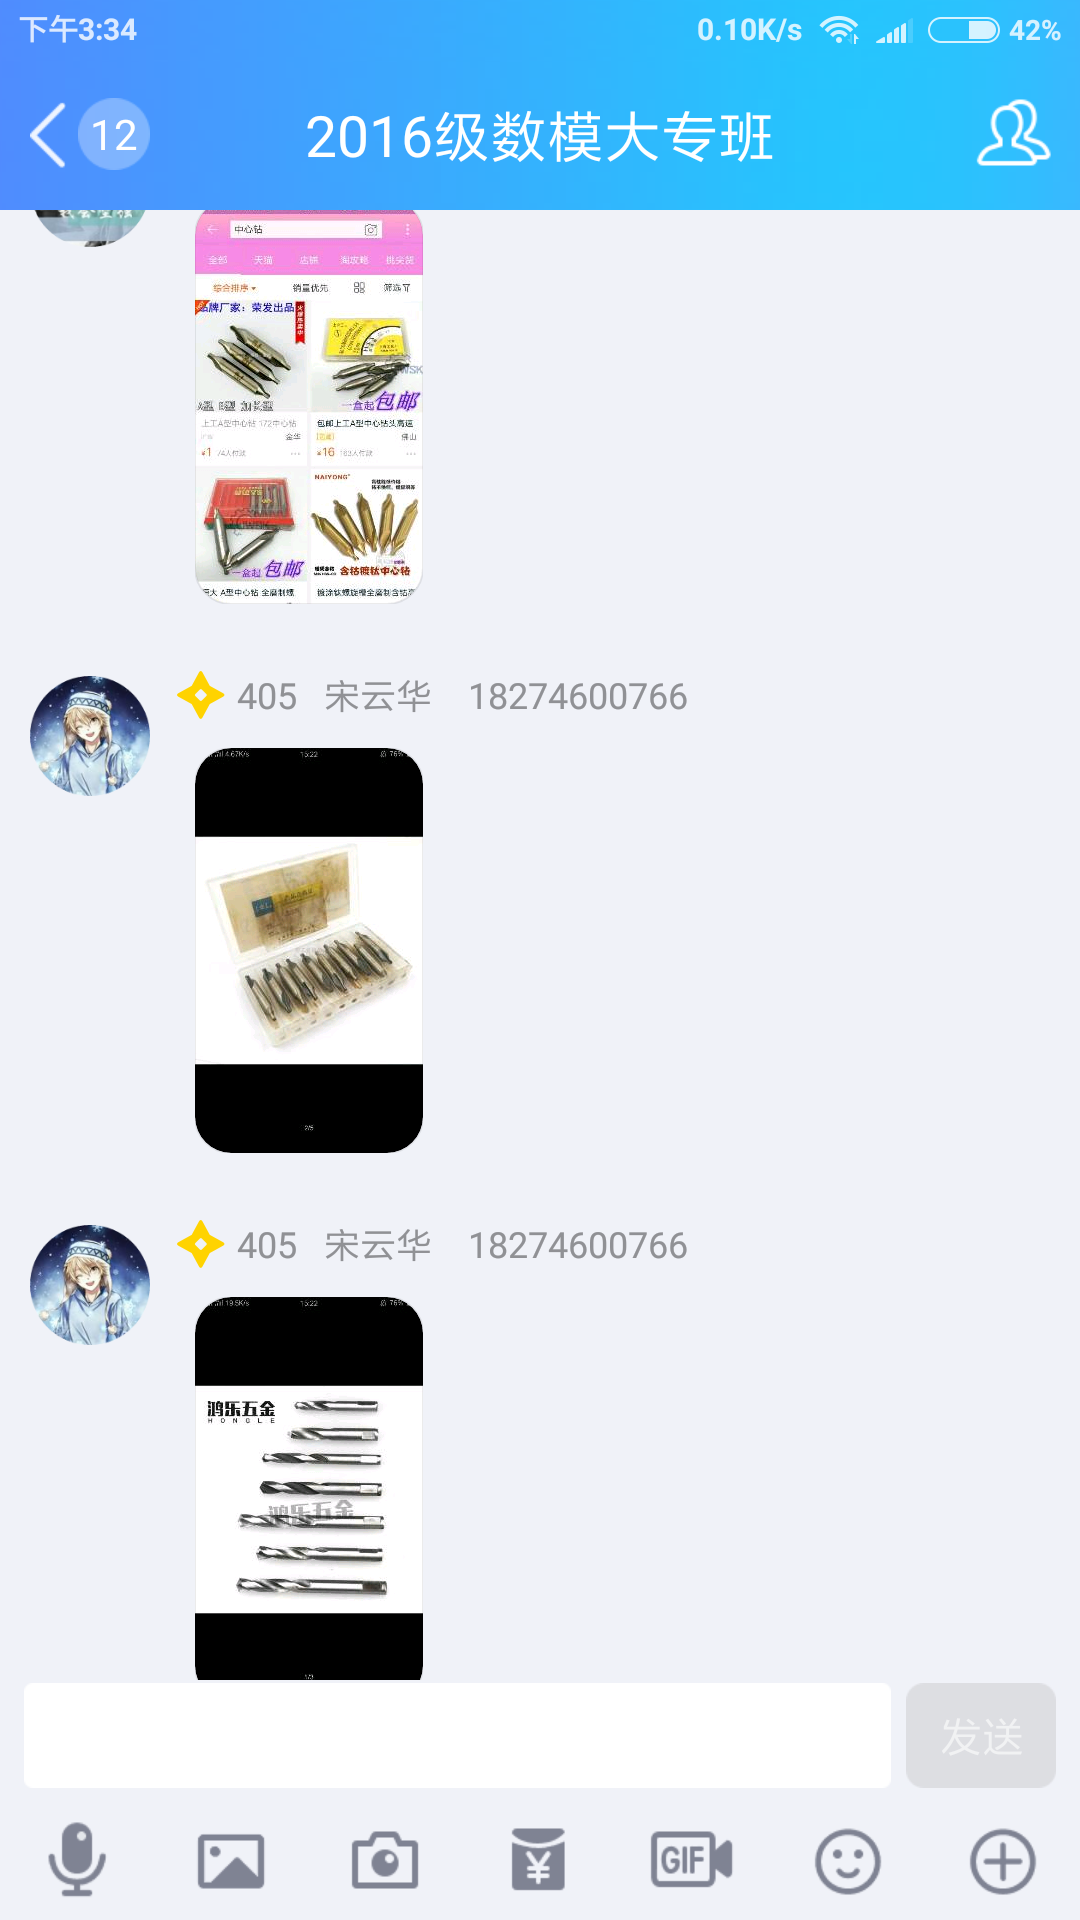
\includegraphics[width=0.2\linewidth,trim=0 0 0 0,clip,angle=0]{image/22}~
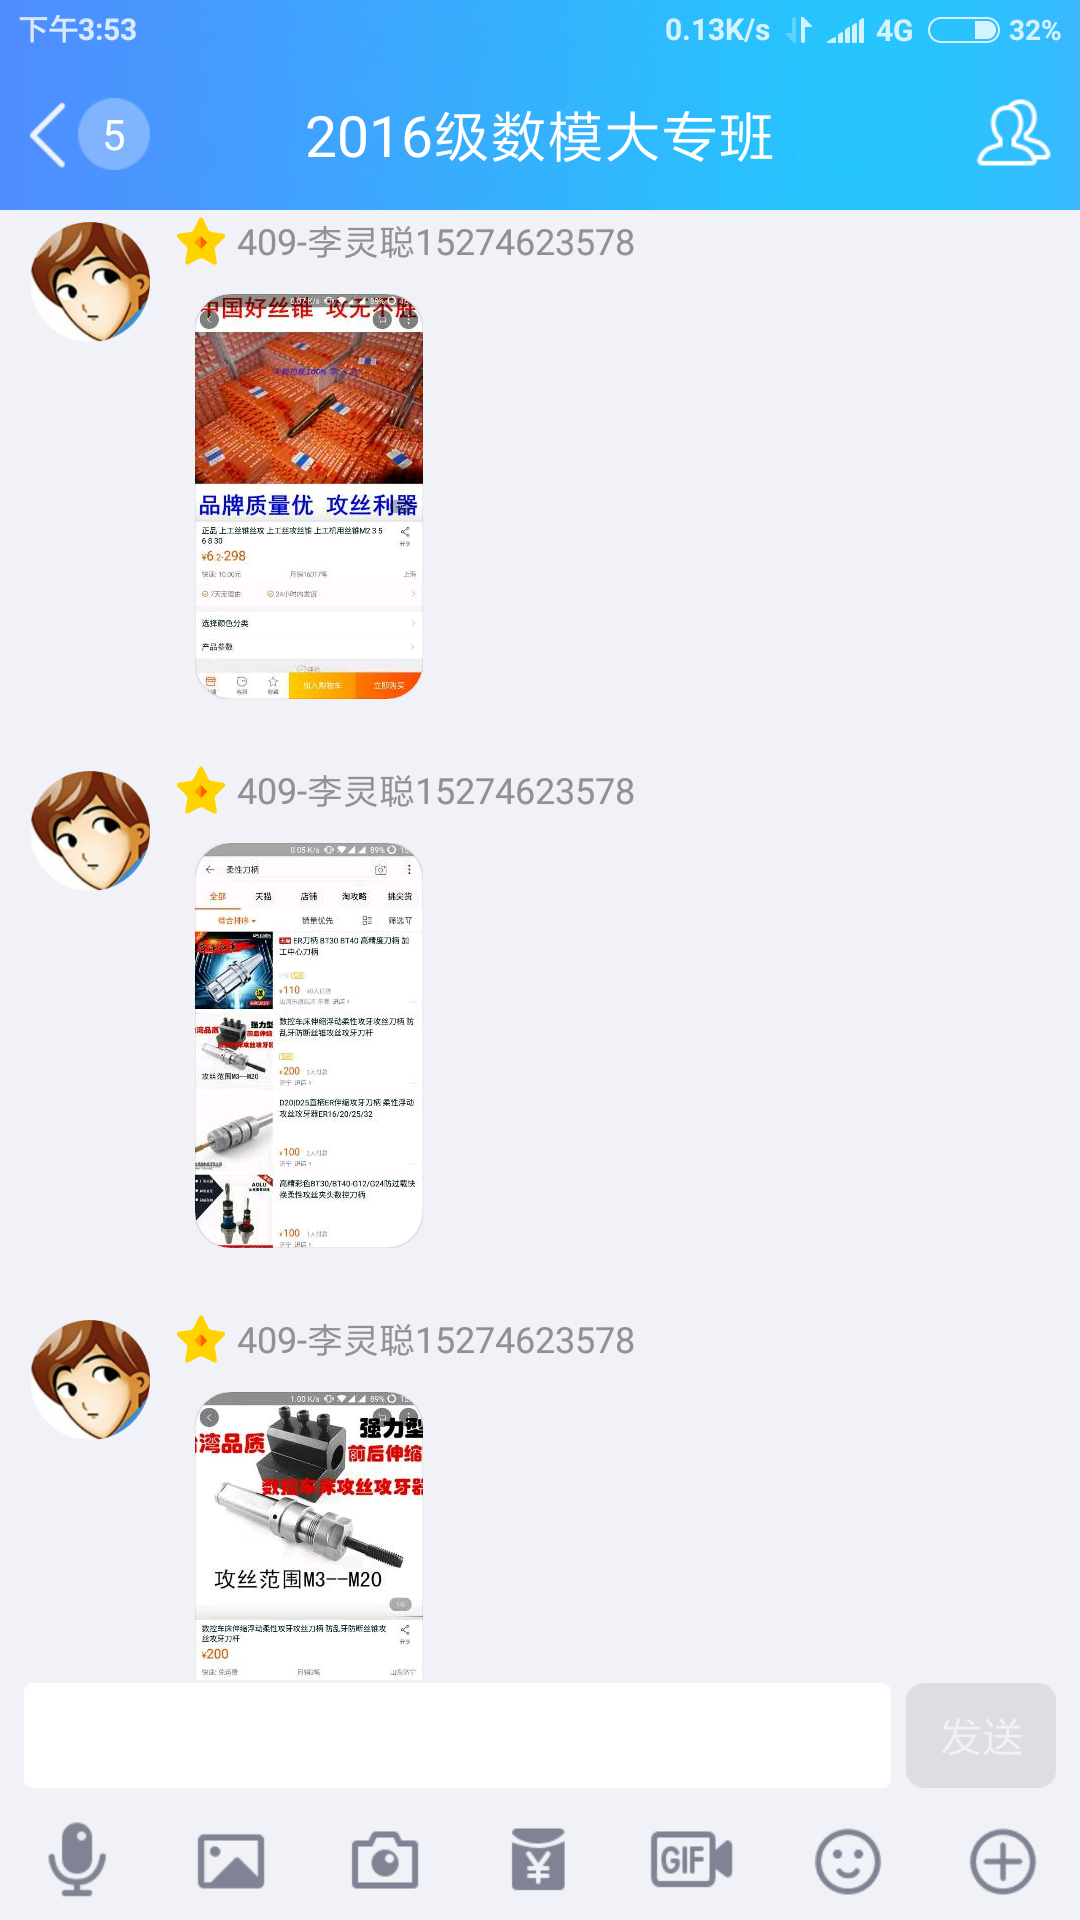
\includegraphics[width=0.2\linewidth,trim=0 0 0 0,clip,angle=0]{image/23}~
\end{frame}

\begin{frame}{铣孔与传统孔加工}
	\begin{columns}
		\column{0\textwidth}
		\column{\textwidth}
		
		视频演示、分析讨论引导。
		
		提问,为什么要用那么多的刀具传统加工孔
		
		引导学生思考:成形原理,受力方向,精度,应用场合。
		\column{0\textwidth}
	\end{columns}
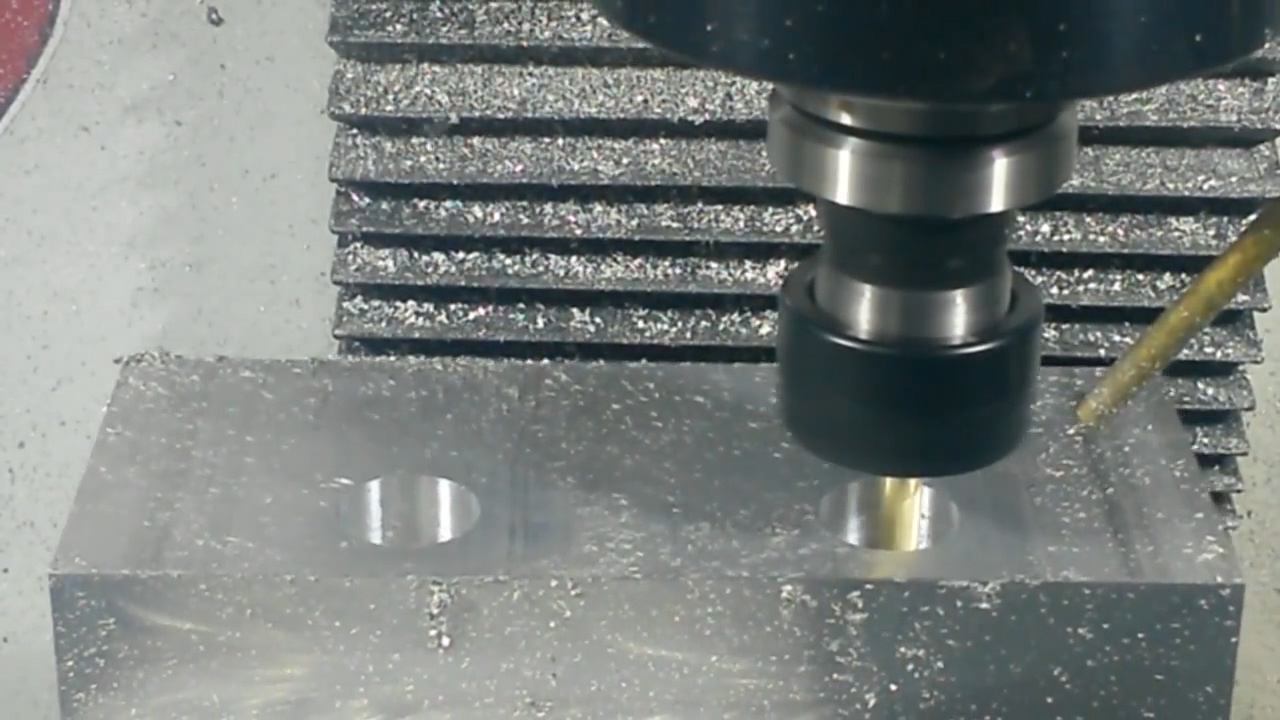
\includegraphics[width=.5\linewidth,trim=0 0 0  0,clip,angle=0]{image/2-1.jpg}~
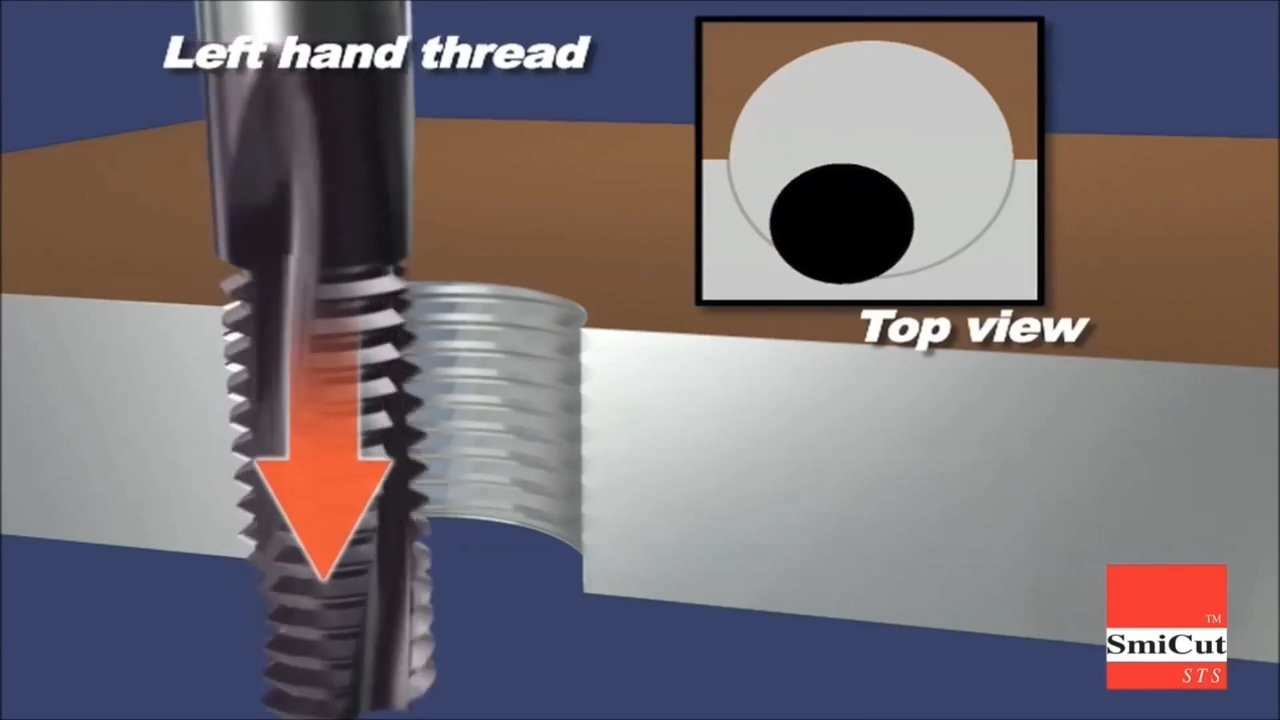
\includegraphics[width=.5\linewidth,trim=0 0 0  0,clip,angle=0]{image/xiluowen2.jpg}~

\end{frame}

\begin{frame}{孔加工的6个步骤与三个平面}
	\begin{columns}
		\column{.5\textwidth}
				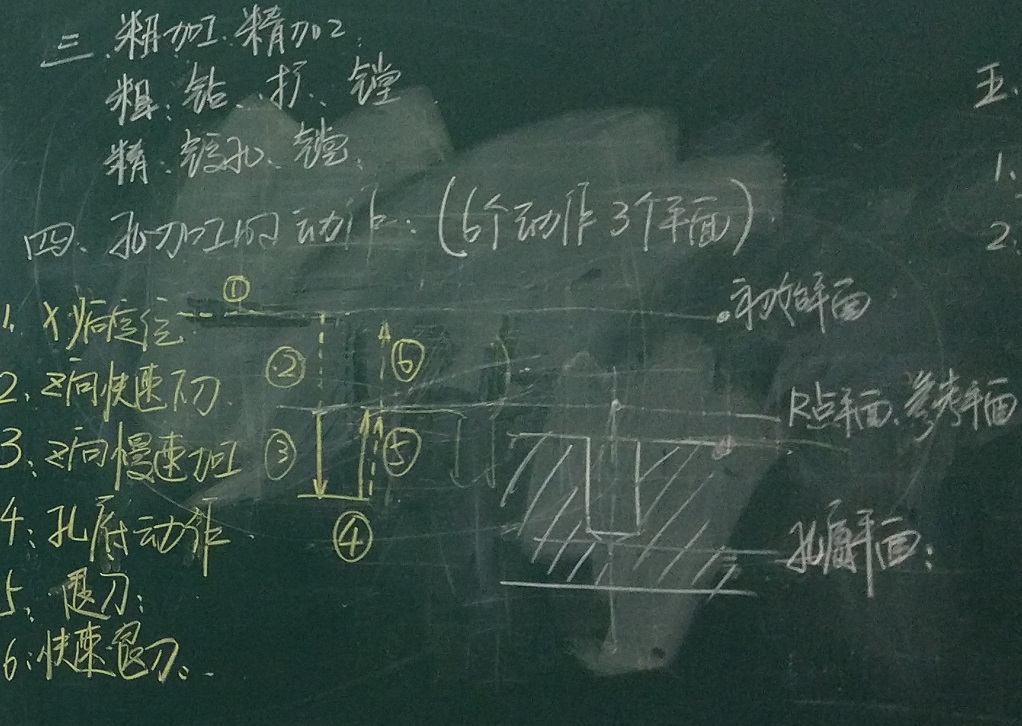
\includegraphics[width=\linewidth,trim=0 0 0 0 ,clip,angle=0]{image/44.jpg}~
		\column{.5\textwidth}
		
		总结、视频回放、引导分析、画图。
		
		孔加工的6个步骤
		
		编程的三个平面以及与加工孔的关系。
		
		\column{0\textwidth}
	\end{columns}
\end{frame}

\begin{frame}{孔加工编程}
	\begin{columns}
		\column{0\textwidth}
		\column{.5\textwidth}
		
		模仿法:
		
\begin{itemize}
	\item 	教师分析每一个过程,
	
	\item 编写第一个孔的程序
	
	\item 学生模仿编写第二个孔加工程序。
	
	\item 找规律,用子程序
	
	\item 模仿使用增量编写。
	
	\item (仿真)
\end{itemize}
	
		\column{0.5\textwidth}
		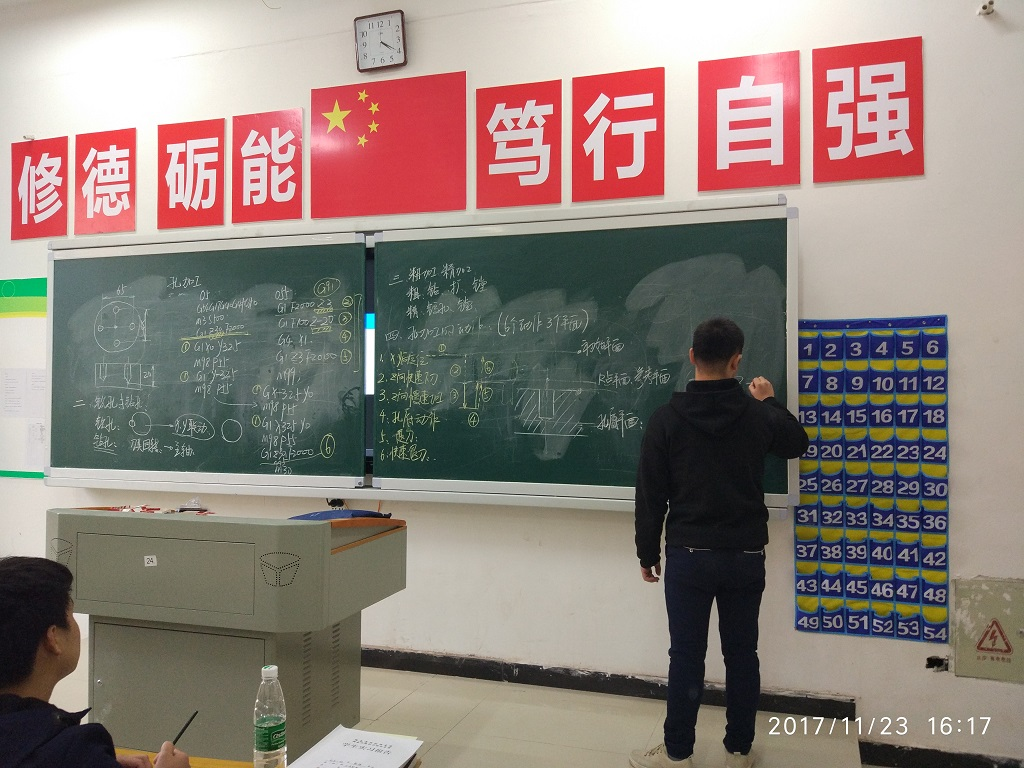
\includegraphics[width=\linewidth,trim=0 0 0  0,clip,angle=0]{image/31.jpg}~
	\end{columns}

\end{frame}

\begin{frame}{小结作业}
	\begin{columns}
		\column{0\textwidth}
		\column{.5\textwidth}
		
		请学生自己总结;
		
	   作业:省技能抽查题 H2-6。
		
		\column{0.5\textwidth}
		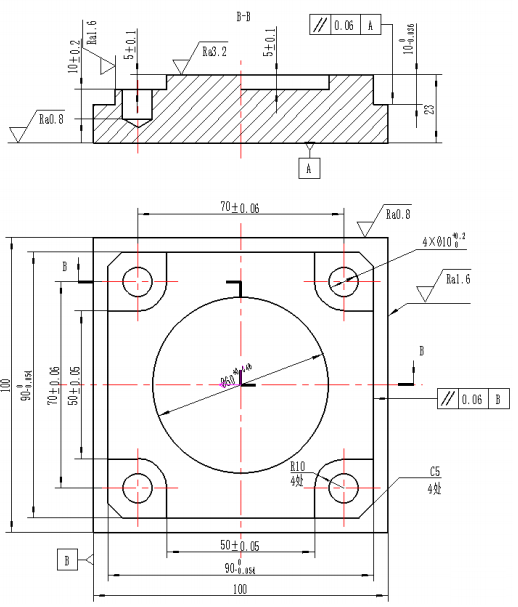
\includegraphics[width=\linewidth,trim=0 0 0  0,clip,angle=0]{image/66}~
	\end{columns}
	
\end{frame}

\section{说教学反思}
\begin{frame}{说教学反思}
    \begin{columns}
        \column{0\textwidth}
        \column{0.5\textwidth}
        
        教学目标反思
          
          达到知识目标、能力目标、情感目标。
          
        教学效果
          
          看视频学生很认真:
                   		
          
          
          学生程序能上电脑上仿真更好
          
          (一体机没有键盘鼠标不好用)  
        
        \column{0.4\textwidth}
        
        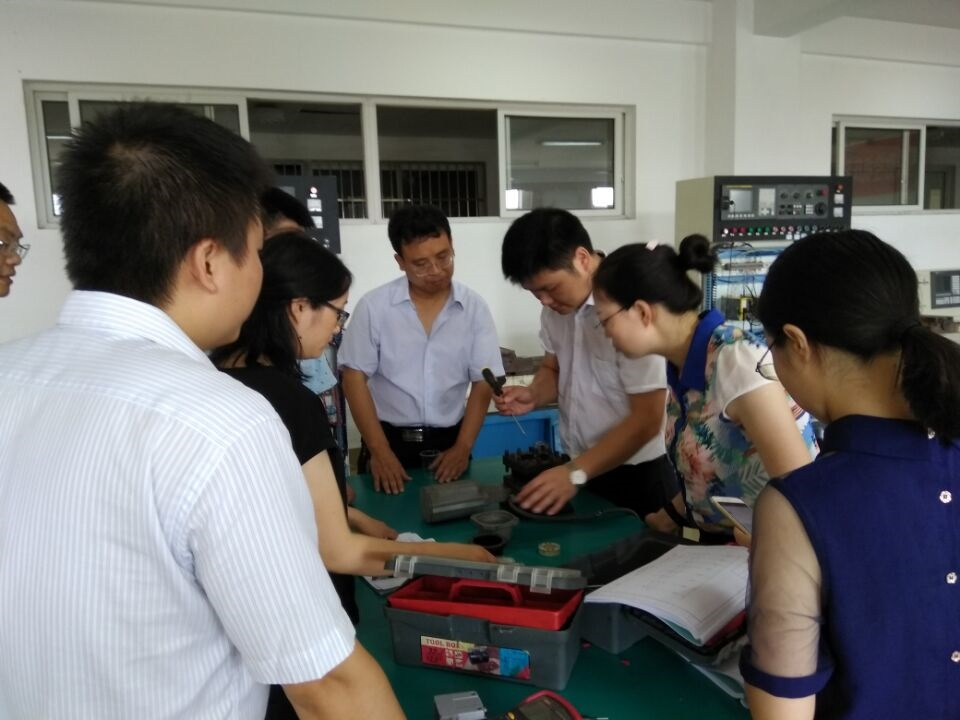
\includegraphics[width=0.7\linewidth,trim=0 0 0  0,clip,angle=0]{image/2}~
        

        \includegraphics[width=0.7\linewidth,trim=0 0 0  0,clip,angle=0]{image/IMG_20171123_162200}
        
        
    \end{columns}

\end{frame}




\section*{感谢}
\begin{frame}[plain]
\vfill

\centering \huge 谢谢大家!

\vfill

\flushleft \footnotesize   
~~~qq:32731964\\
~~~tel:18974681118\\
%~~~课件下载:\\
%~~~https://github.com/gnixoag/myworks2017/tree/master/jiaoshichengzhang

\end{frame}

\section*{模板设计}
%\begin{frame}{模板设计}
%    \begin{center}
%        \smartdiagramset{border color=black,%边界颜色
%            set color list={blue!50!cyan,green!60!lime,orange!50!red,red!80!black},%颜色列表
%            module x sep=5cm,%向间距
%            module y sep=1.5cm,%向间距
%            uniform arrow color=true,%是否制定颜色
%            arrow color=white,%箭头颜色
%            arrow line width=0.5cm,%箭头宽度
%            back arrow disabled=true,%是否箭头返回
%            %   module minimum width=5cm,%最小宽度
%            %module minimum height=2cm,%最小高度
%            text width=4cm,%文本宽度
%        }
%        %\smartdiagram[circular diagram]{一,二,三,四,五}%圆形,逆时针。
%        %\smartdiagram[circular diagram:clockwise]{一,二,三,四,五}%圆形,顺时针。
%        %\smartdiagram[flow diagram]{一,二,三,四,五}%垂直流线。
%        %\smartdiagram[flow diagram:horizontal]{一,二,三,四,五}%水平流线。
%        %\smartdiagram[descriptive diagram]{{一,{一一}},{二,{二二}},{三,{三三}},{四,{四四}},{五,{五五}}}%详细
%        %\smartdiagram[priority descriptive diagram]{一,二,三,四,五}%层次详细
%        \smartdiagram[bubble diagram]{数控铣编程与操作,基本知识,平面加工,外形加工,挖槽加工,孔加工,简化编程}%中心主题
%        %\smartdiagram[constellation diagram]{一,二,三,四,五}%中心主题,带箭头。
%        %\smartdiagram[connected constellation diagram]{一,二,三,四,五}%中心主题,子项相连。
%        %\smartdiagram[sequence diagram]{{一,{一一}},{二,{二二}},{三,{三三}},{四,{四四}},{五,{五五}}}%箭头向前。
%    \end{center}
    
%\end{frame}

%\AtBeginSection{
%    \begin{frame}{说课内容}
%        \begin{columns}[onlytextwidth]
%            \column[c]{0.1\textwidth}	
%            \column[c]{0.3\textwidth}
%            \tableofcontents[currentsection,hideallsubsections]
%            \column[c]{0.6\textwidth}
%            \vspace{0.5cm}
%            \includegraphics[width=0.9\linewidth,trim=0 0 0 0,clip,angle=0]{image/2.jpg}
%        \end{columns}
%    \end{frame}
%}

%\begin{frame}{说教学反思}
%    \begin{columns}
%        \column{0\textwidth}
%        \column{\textwidth}
%        \column{0\textwidth}
%    \end{columns}
%\end{frame}

\end{document} 
